This chapter dives deep into how Students\&Companies is implemented, integrated and tested.
The chosen approach follows a bottom-up strategy.
It begins with developing and testing foundational elements before integrating the rest of the system.
This gradual process focuses on the independent development of basic modules, which are tested in isolation before being integrated into the larger system.
This independence eliminates the need to consider the entire system upfront, making it easier and faster to address issues and apply changes.
A key factor of this method is the use of drivers, which are tests that simulate the inputs essential for validating individual modules.

\section{Test Plan}
Following the bottom-up strategy, a layered testing plan is employed to ensure system reliability.
Unit tests use drivers to simulate inputs for individual submanagers, verifying their functionality in isolation.
As modules are progressively integrated, integration tests verify the interactions between components, such as database queries, ensuring that combined functionalities work as expected.
Once a manager is fully integrated, functional tests are performed to guarantee the alignment with the functionalities, goals and constraints outlined in the requirements analysis and specification document \cite{carraracurrodossi2024}.
To assess the system's ability to handle real-world demands, load testing evaluates the platform's performance under normal and peak traffic conditions, while performance testing measures responsiveness, ensuring the system meets the required standards for speed.

\section{Implementation and Integration}
The plan begins with the development and testing of base components, specifically the foundational submanagers within each manager.
Once these base submanagers are implemented and tested, the remaining ones for the same manager are integrated. 
To ensure clarity, when all submanagers of a manager are integrated, they are represented in the diagrams through their respective manager component.

\clearpage
The first step is to implement and test the model.

\begin{figure}[h]
    \centering
    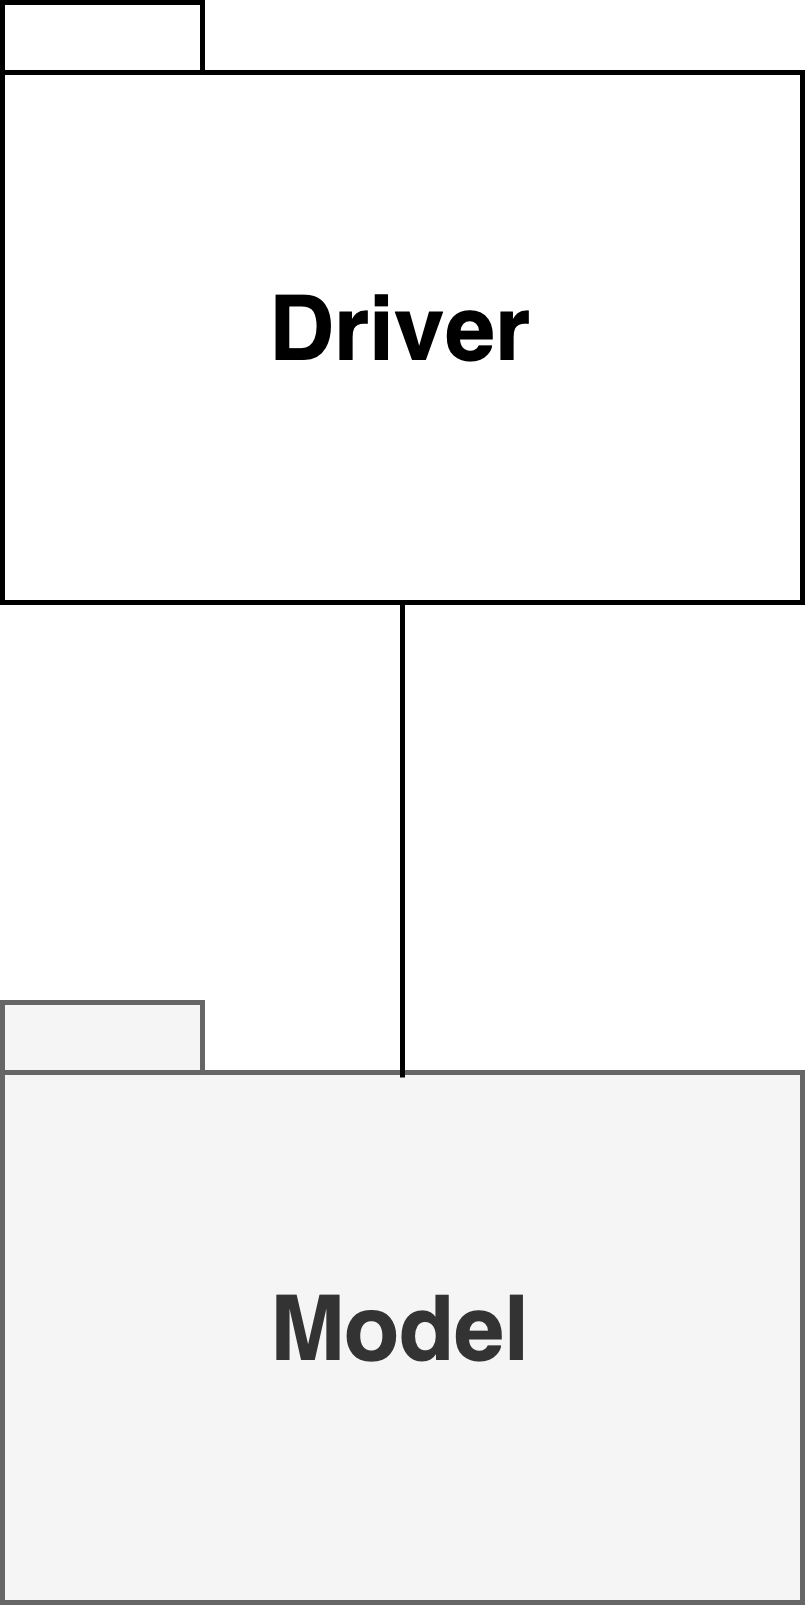
\includegraphics[width=2.5cm]{images/implementation-steps/1.png}
    \caption{Implementation step 1}
\end{figure}

The development proceeds to step two with the user signup and login submanagers.

\begin{figure}[h]
    \centering
    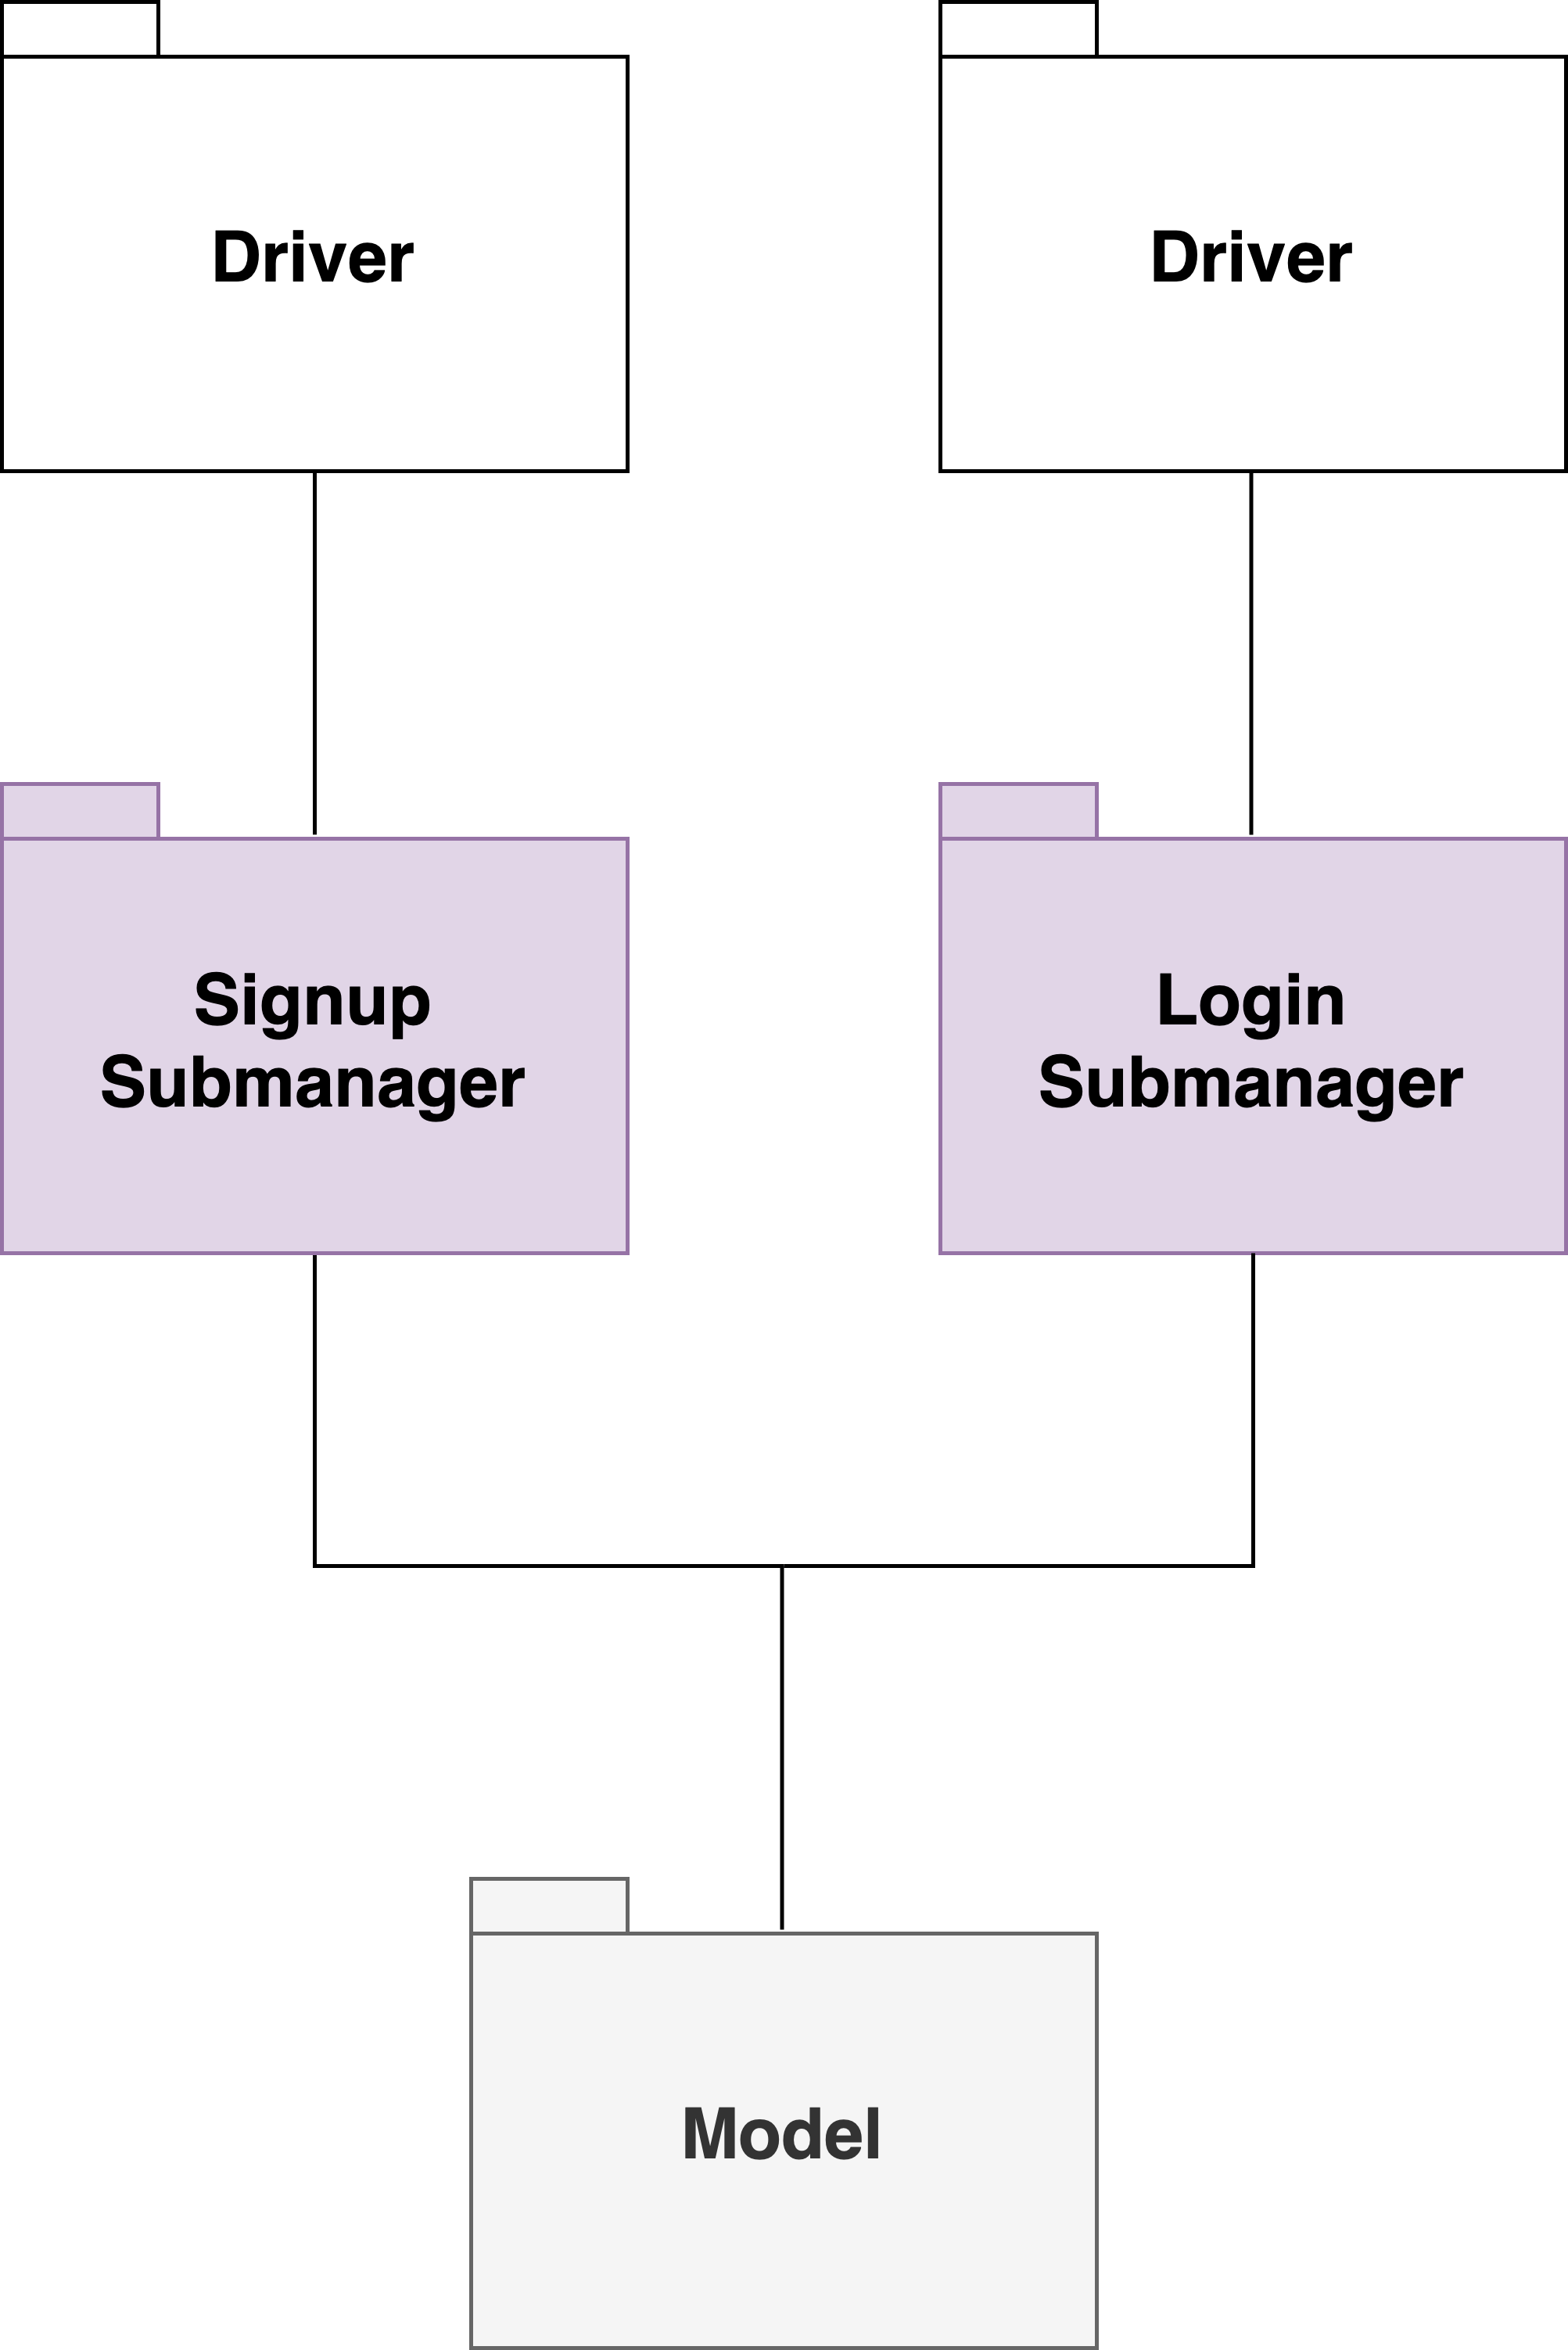
\includegraphics[width=6.5cm]{images/implementation-steps/2.png}
    \caption{Implementation step 2}
\end{figure}

\clearpage
The user management submanager is integrated in the third step.

\begin{figure}[h]
    \centering
    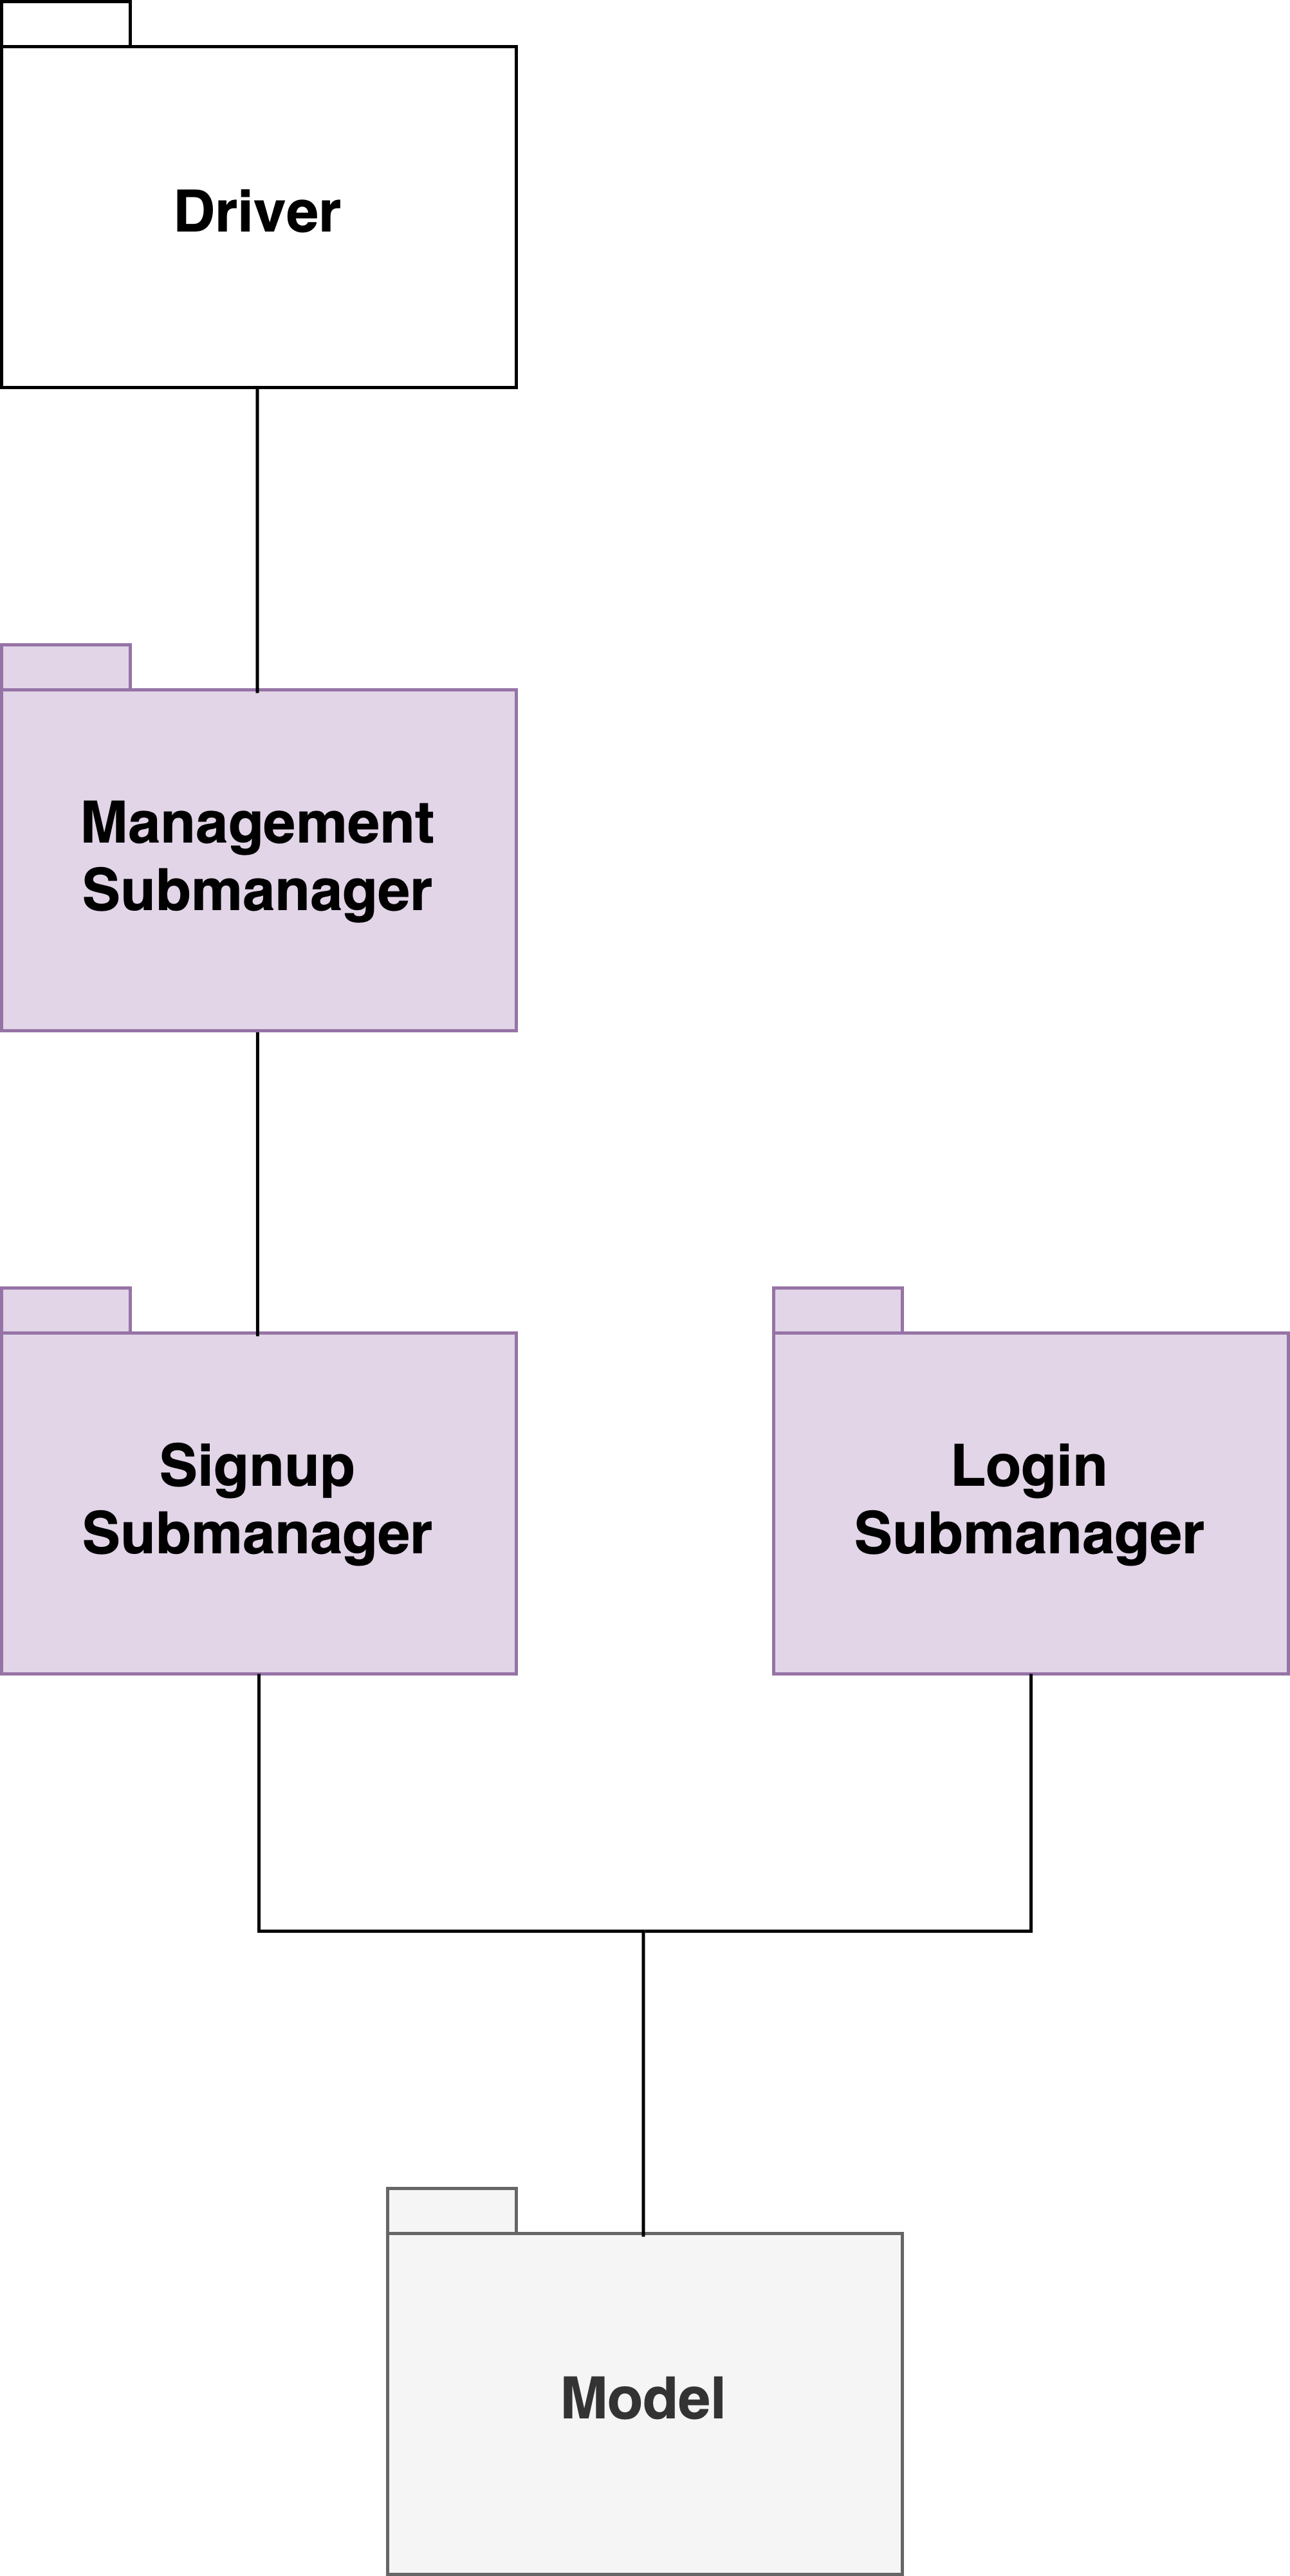
\includegraphics[width=6.5cm]{images/implementation-steps/3.png}
    \caption{Implementation step 3}
\end{figure}

\clearpage
Step four applies the same pattern to the position posting and search submanagers.

\begin{figure}[h]
    \centering
    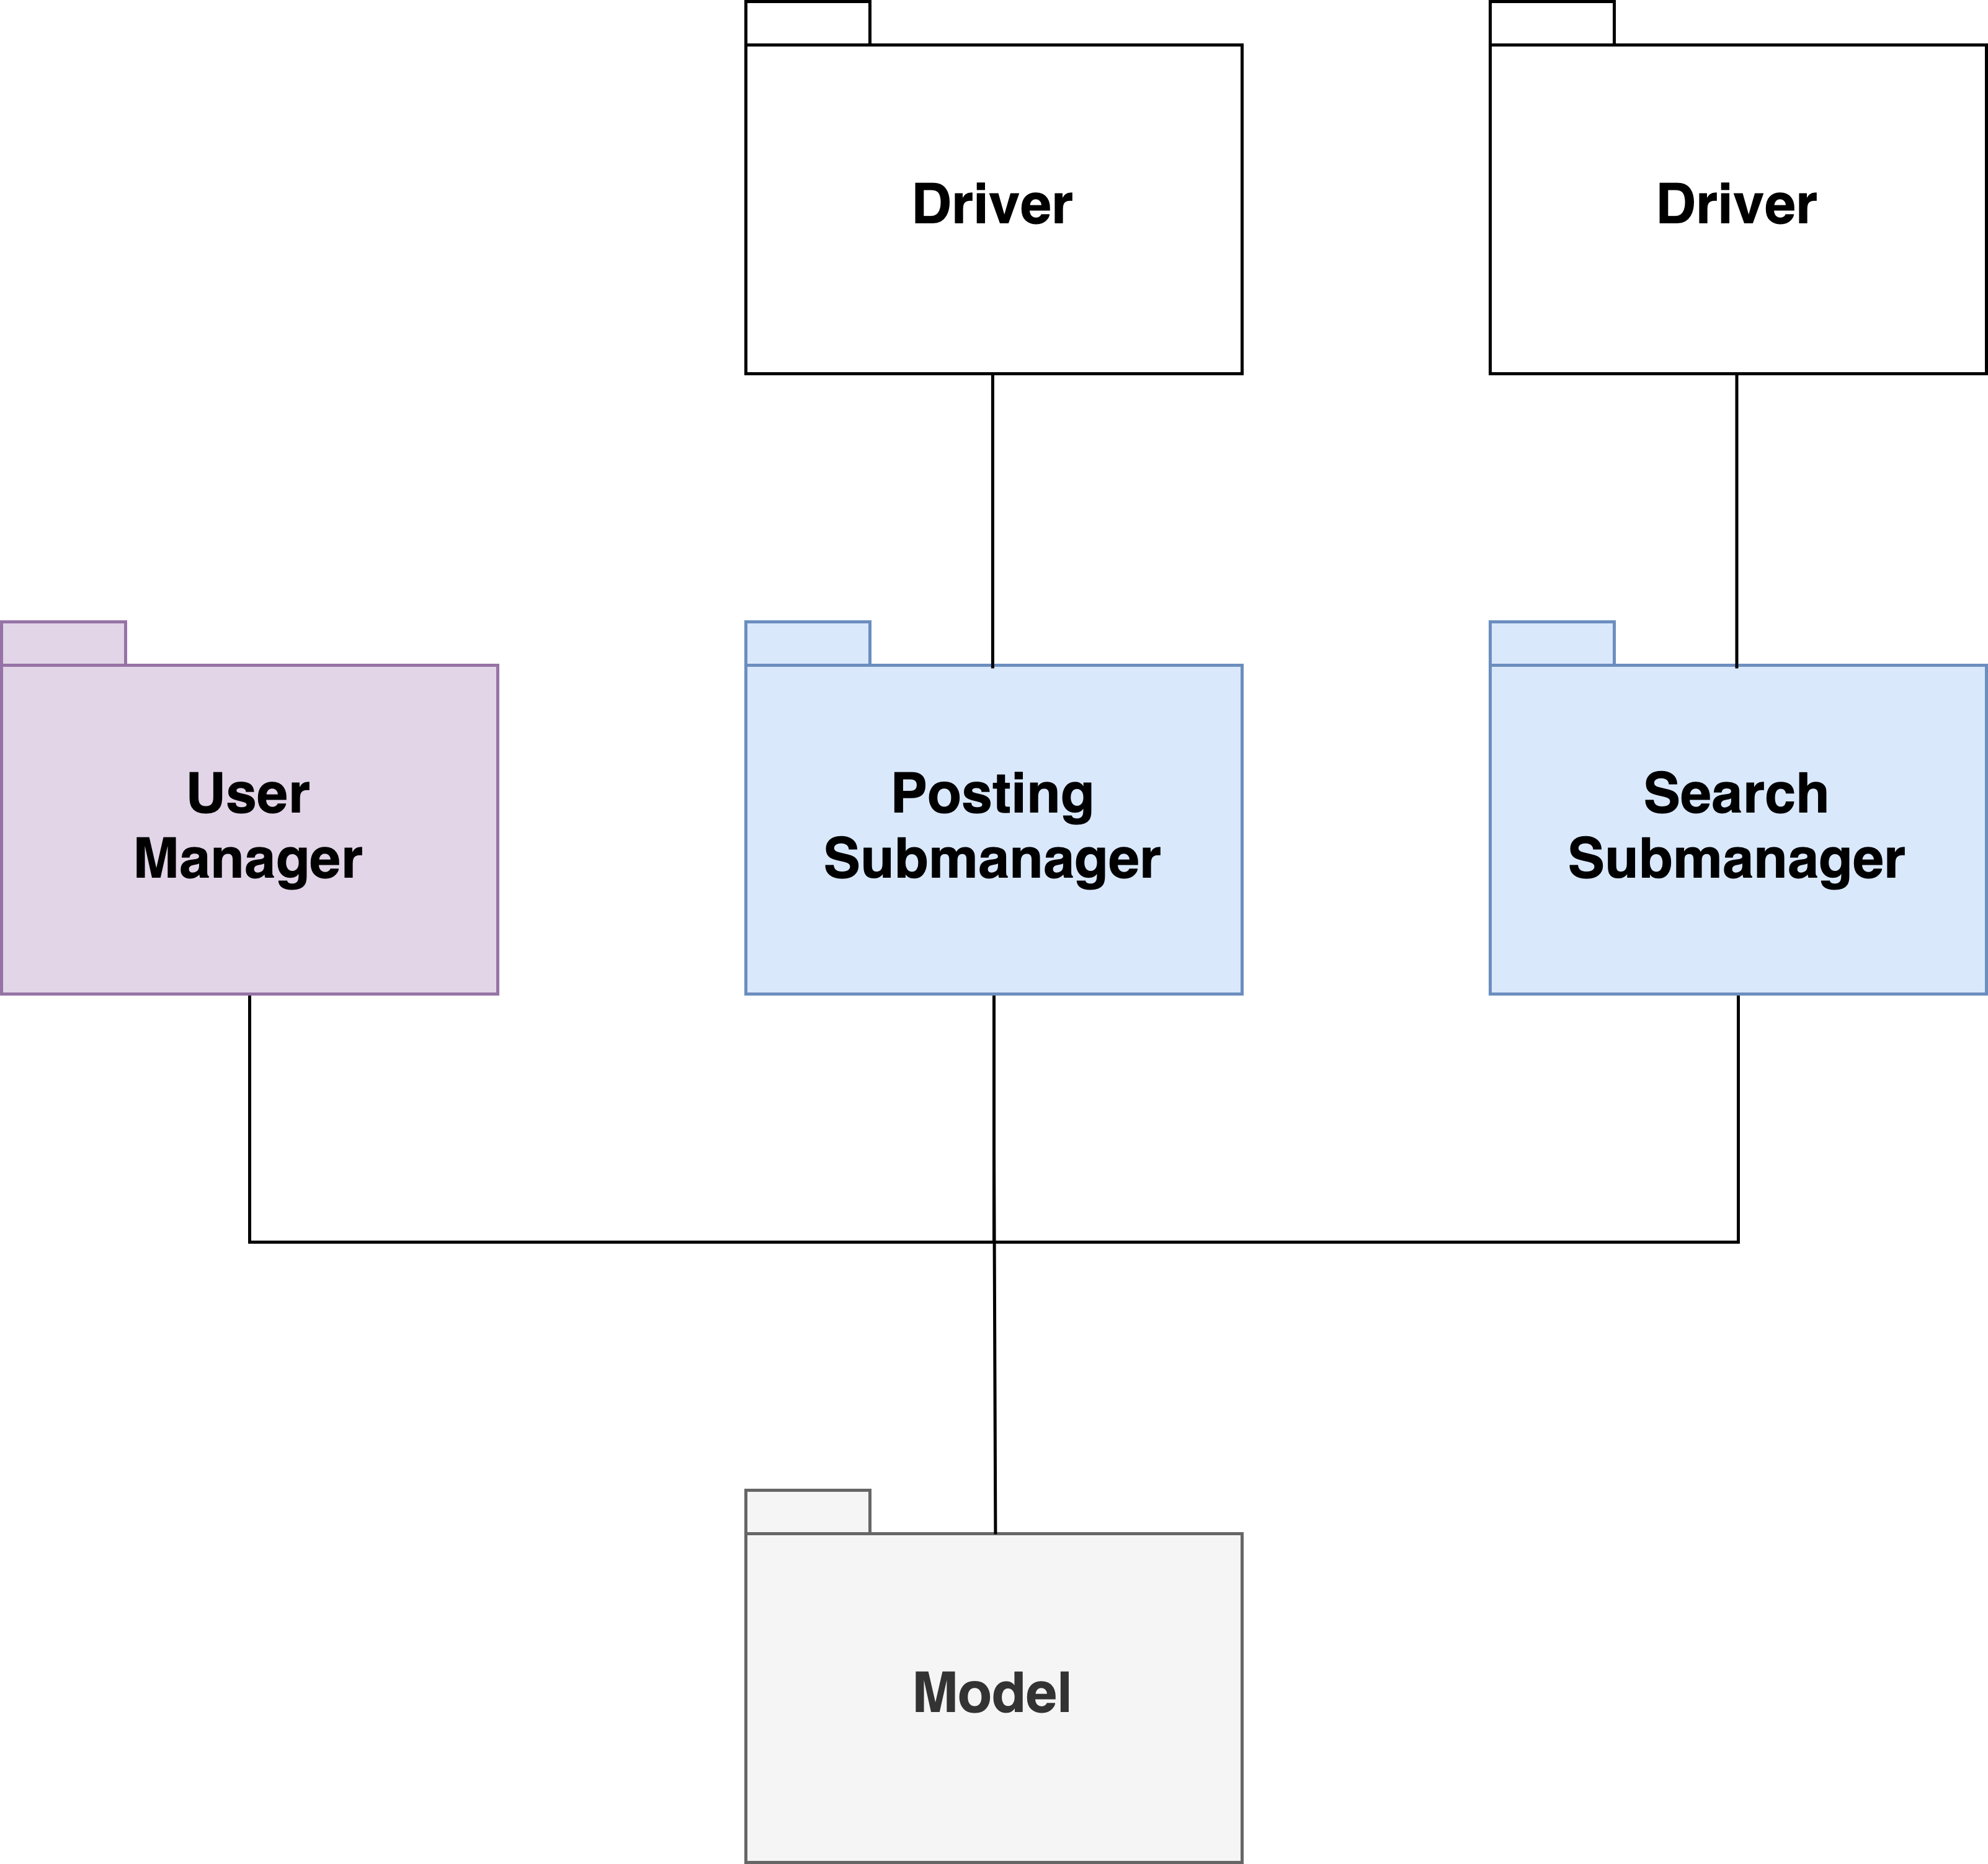
\includegraphics[width=10cm]{images/implementation-steps/4.png}
    \caption{Implementation step 4}
\end{figure}

\clearpage
The position management submanager is integrated in the fifth step.

\begin{figure}[h]
    \centering
    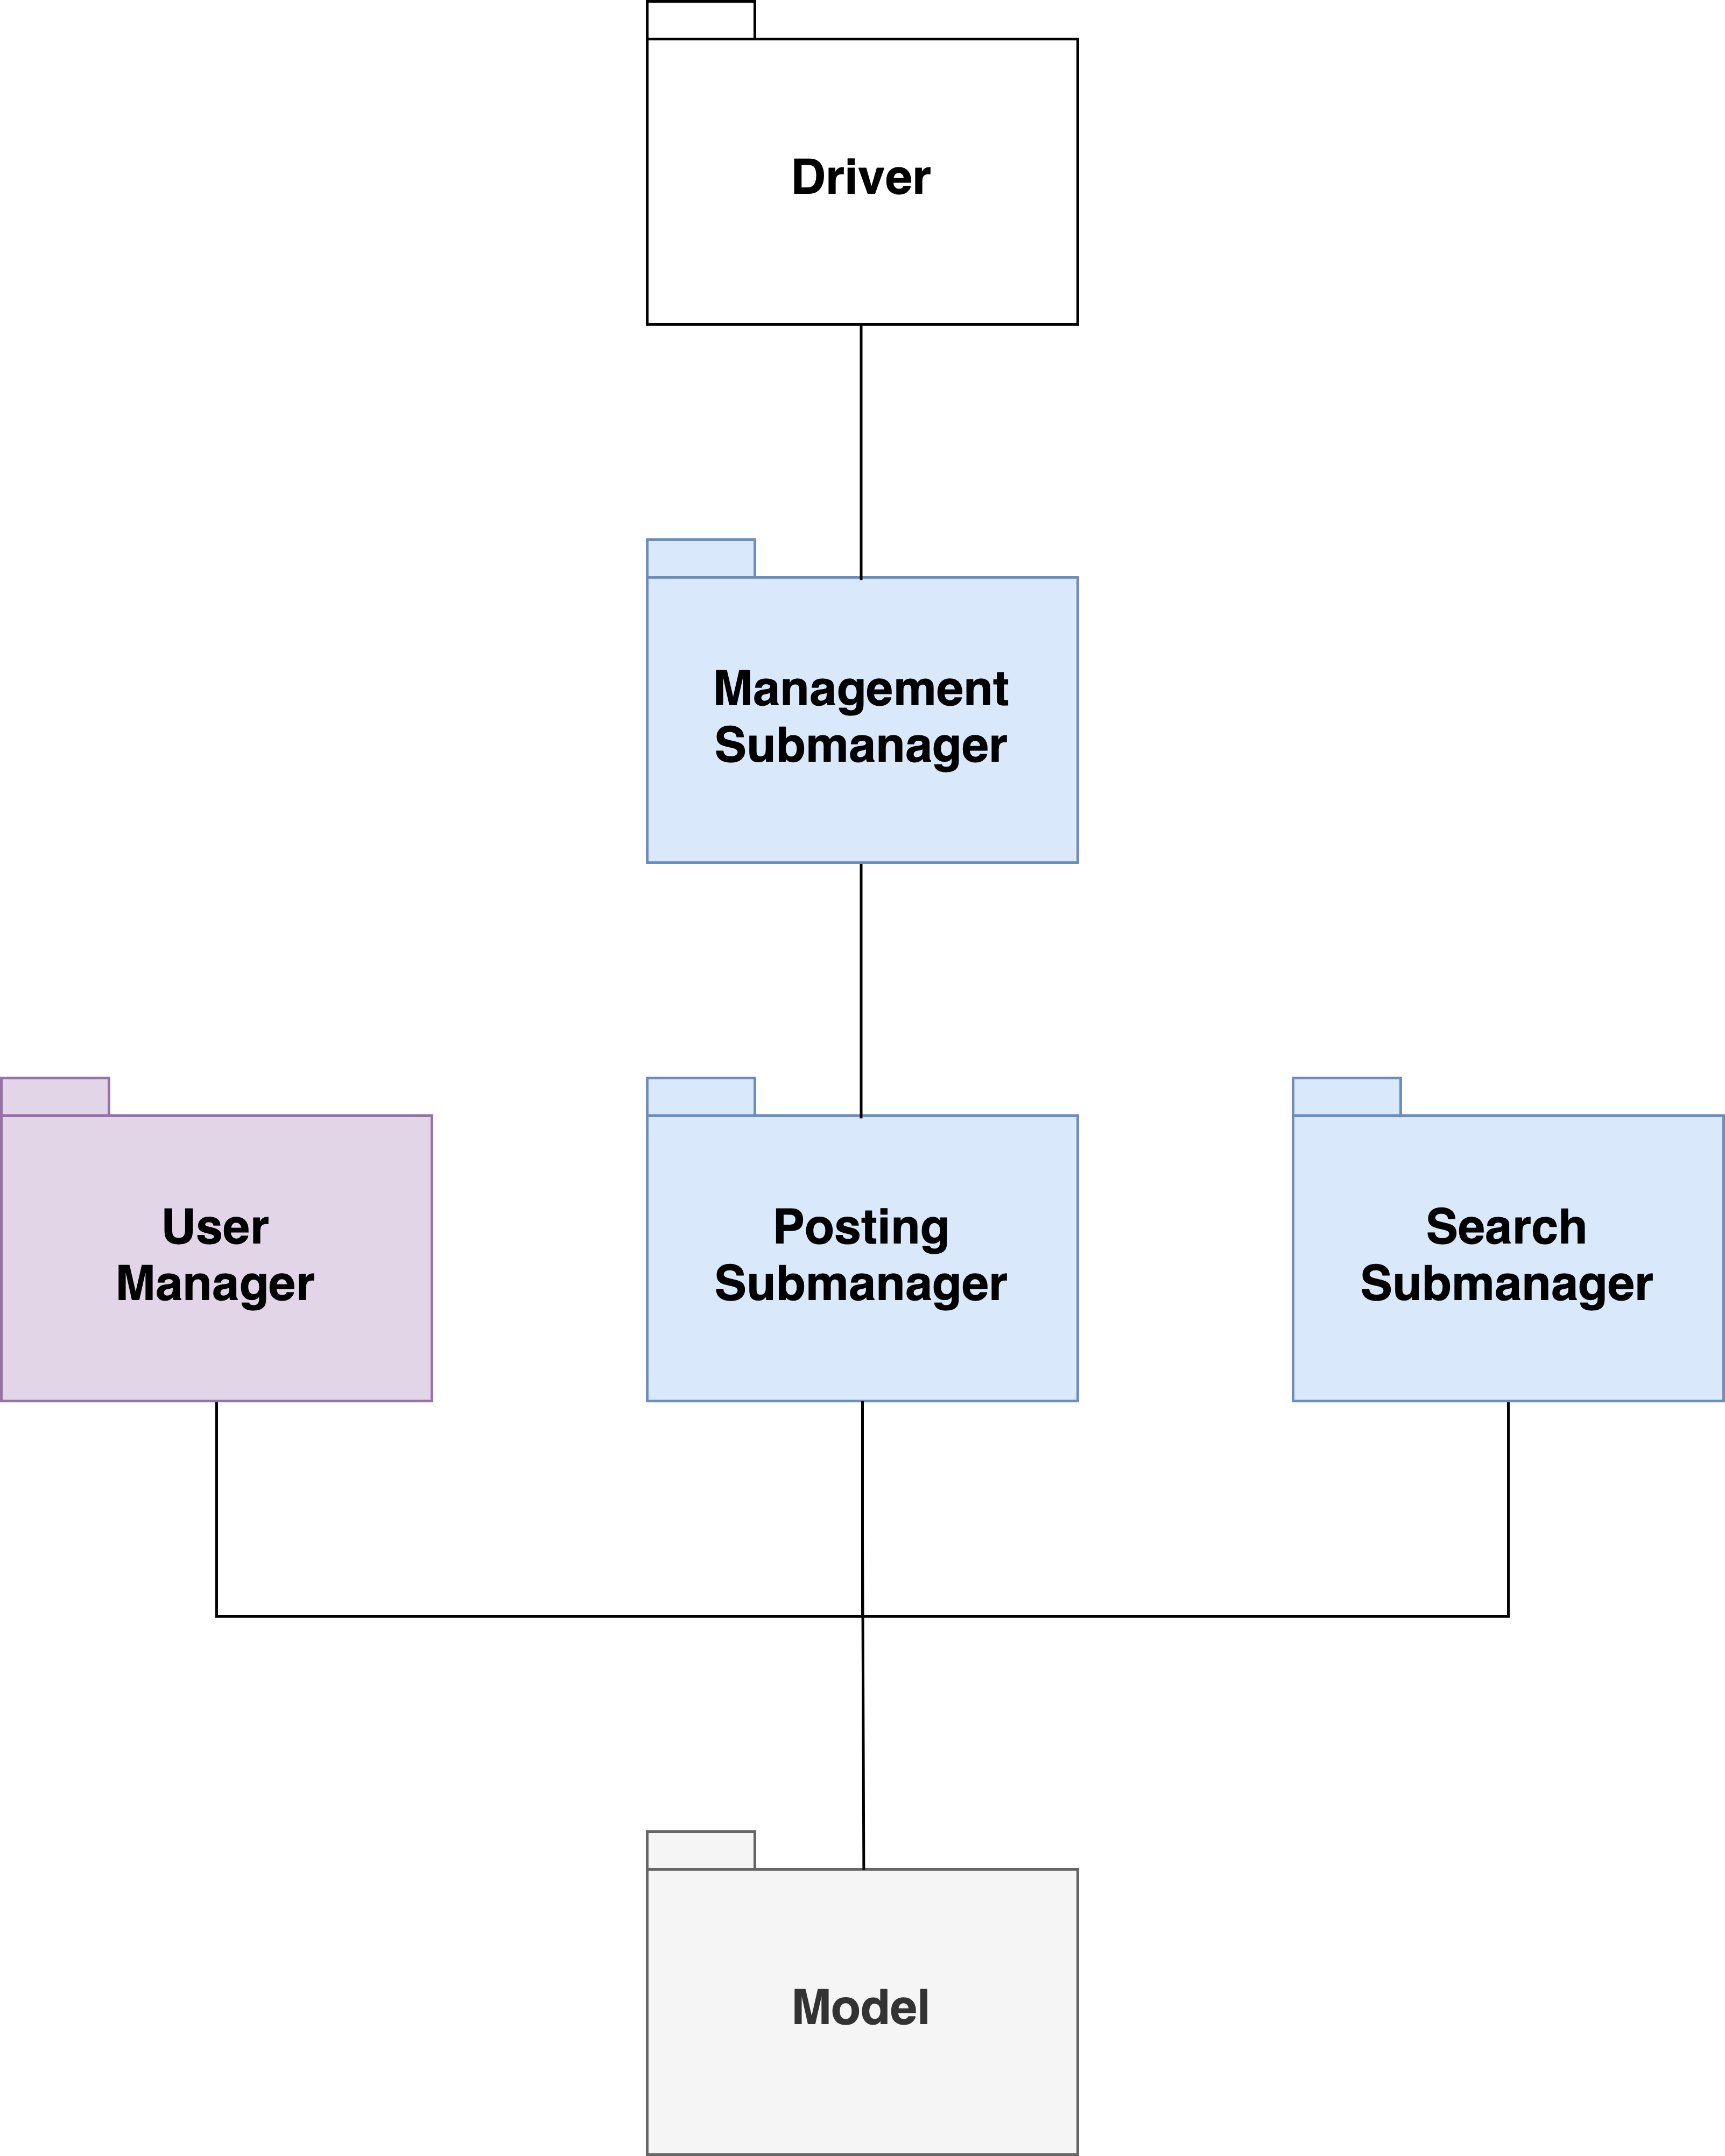
\includegraphics[width=10cm]{images/implementation-steps/5.png}
    \caption{Implementation step 5}
\end{figure}

\clearpage
The development proceeds to step six with the recommendation submanagers.

\begin{figure}[h]
    \centering
    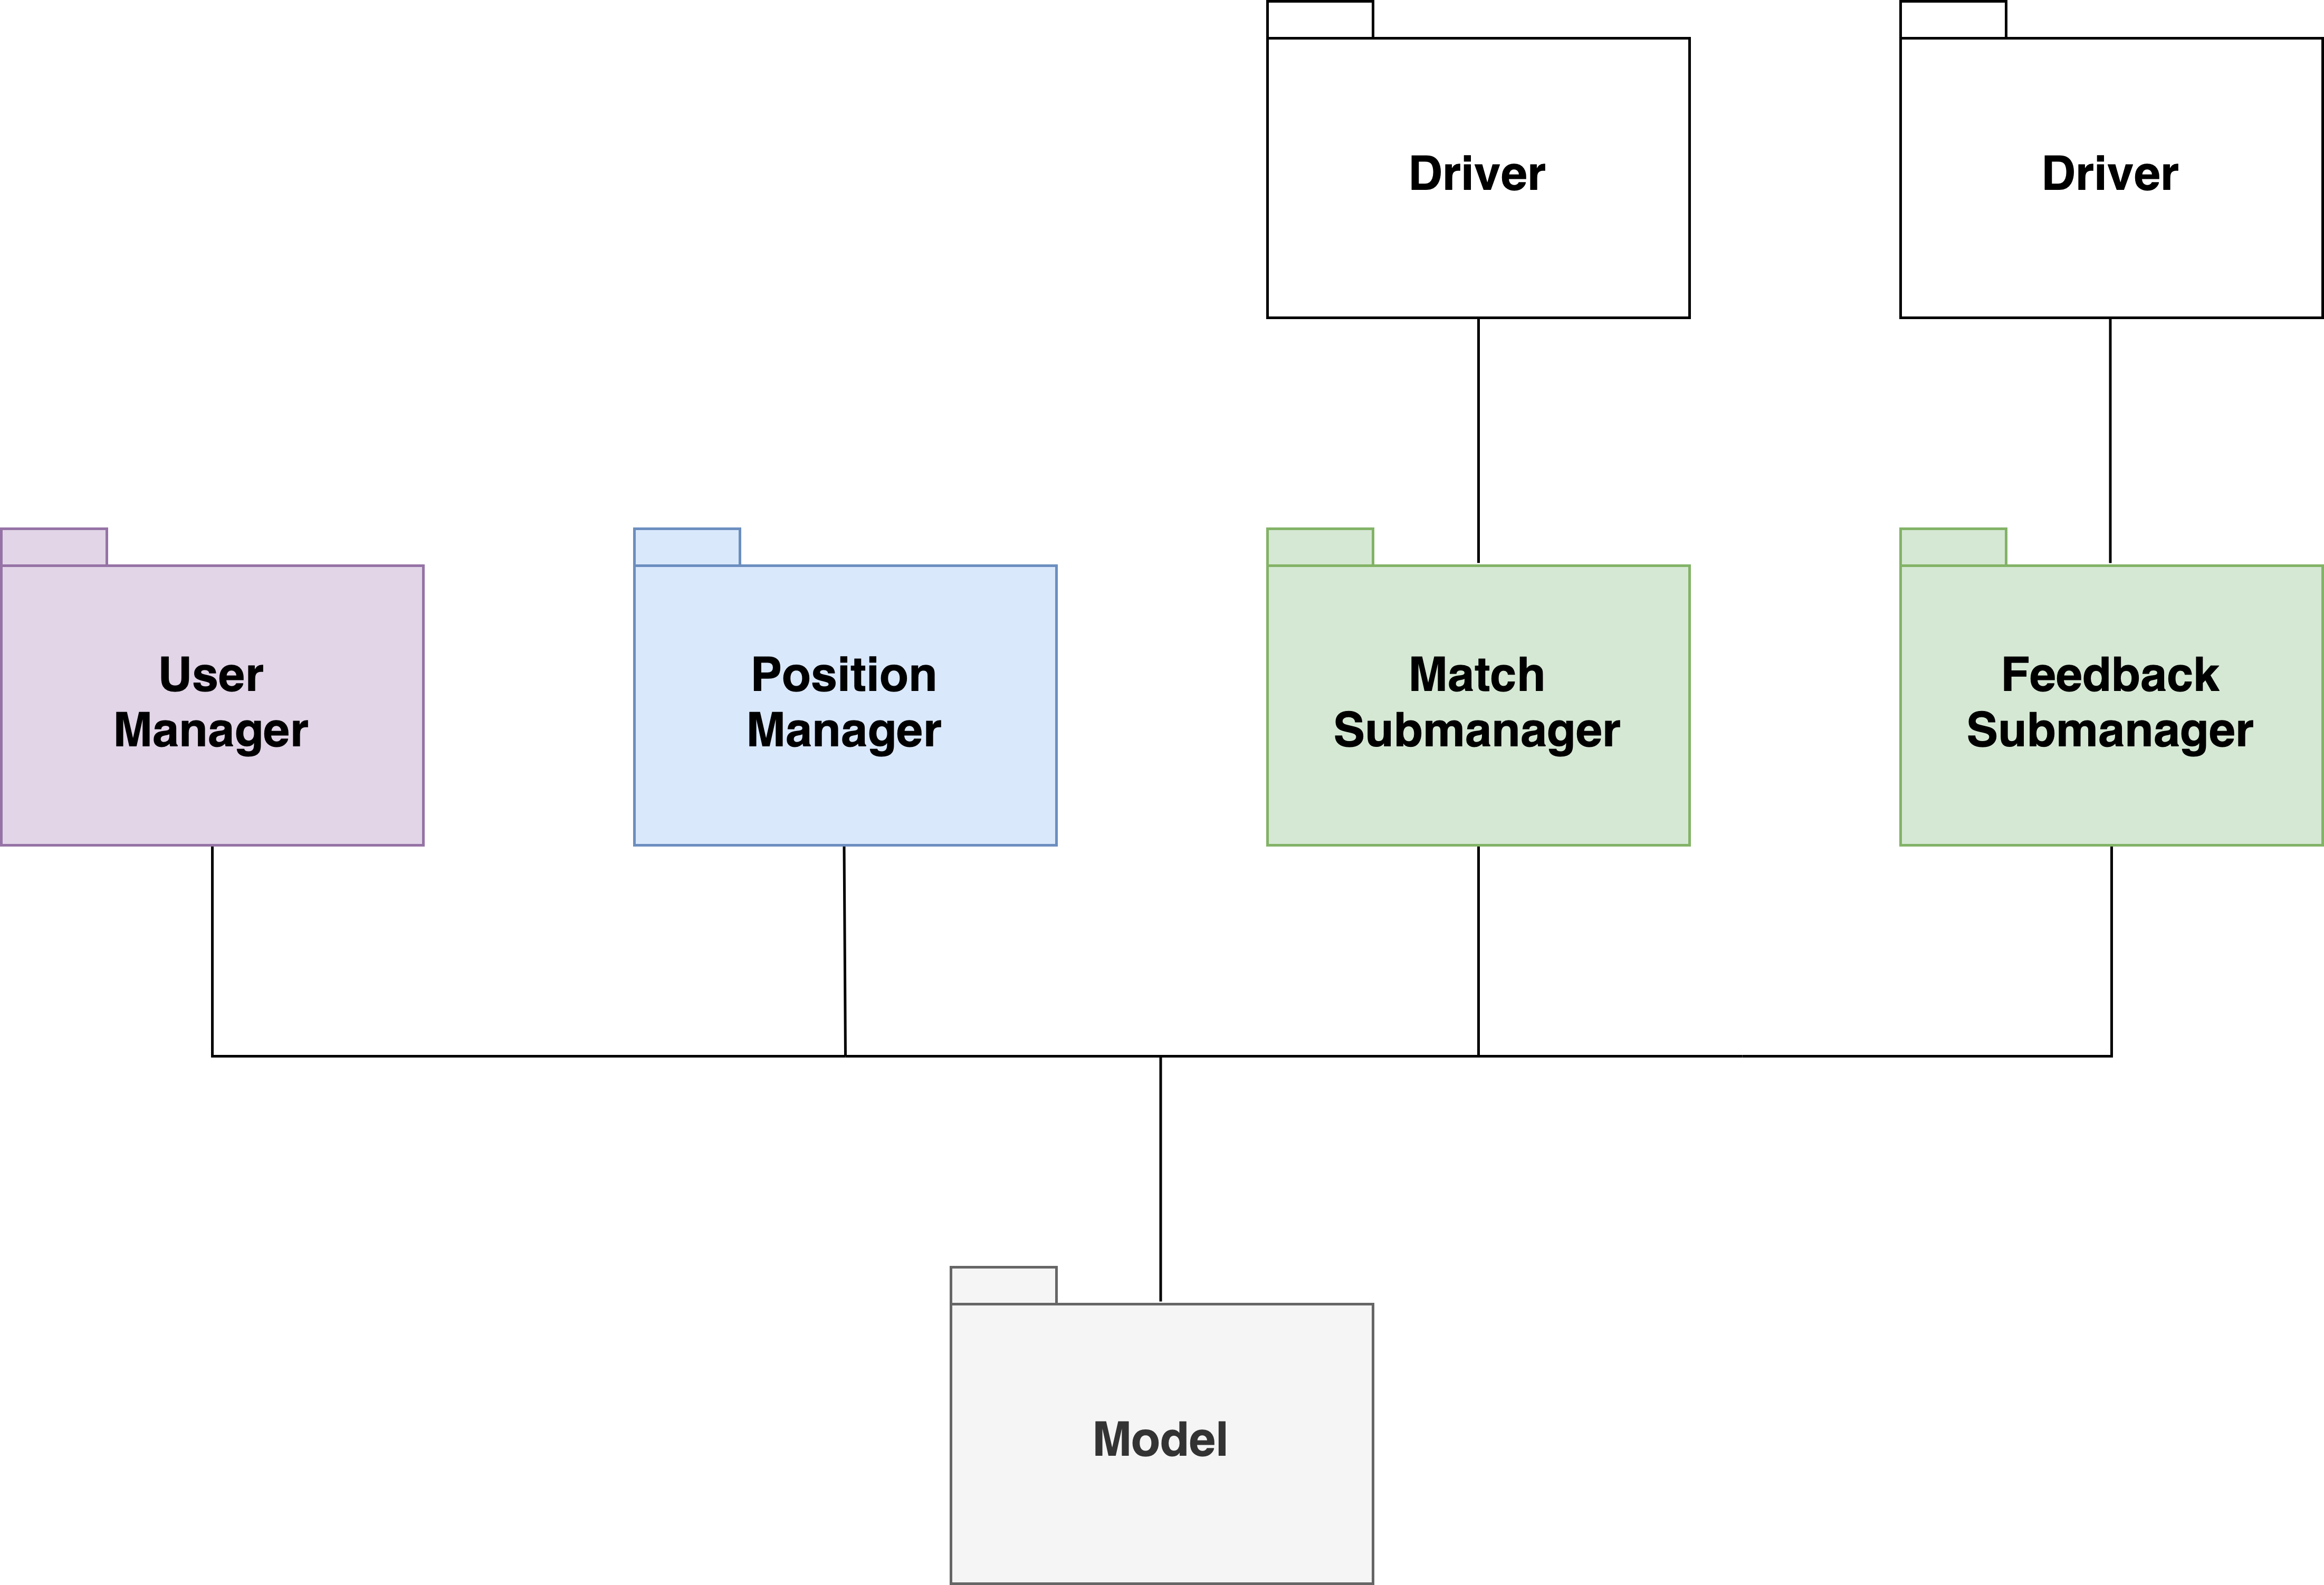
\includegraphics[width=13cm]{images/implementation-steps/6.png}
    \caption{Implementation step 6}
\end{figure}

\clearpage
Step seven applies the same pattern to the selection application submanager.

\begin{figure}[h]
    \centering
    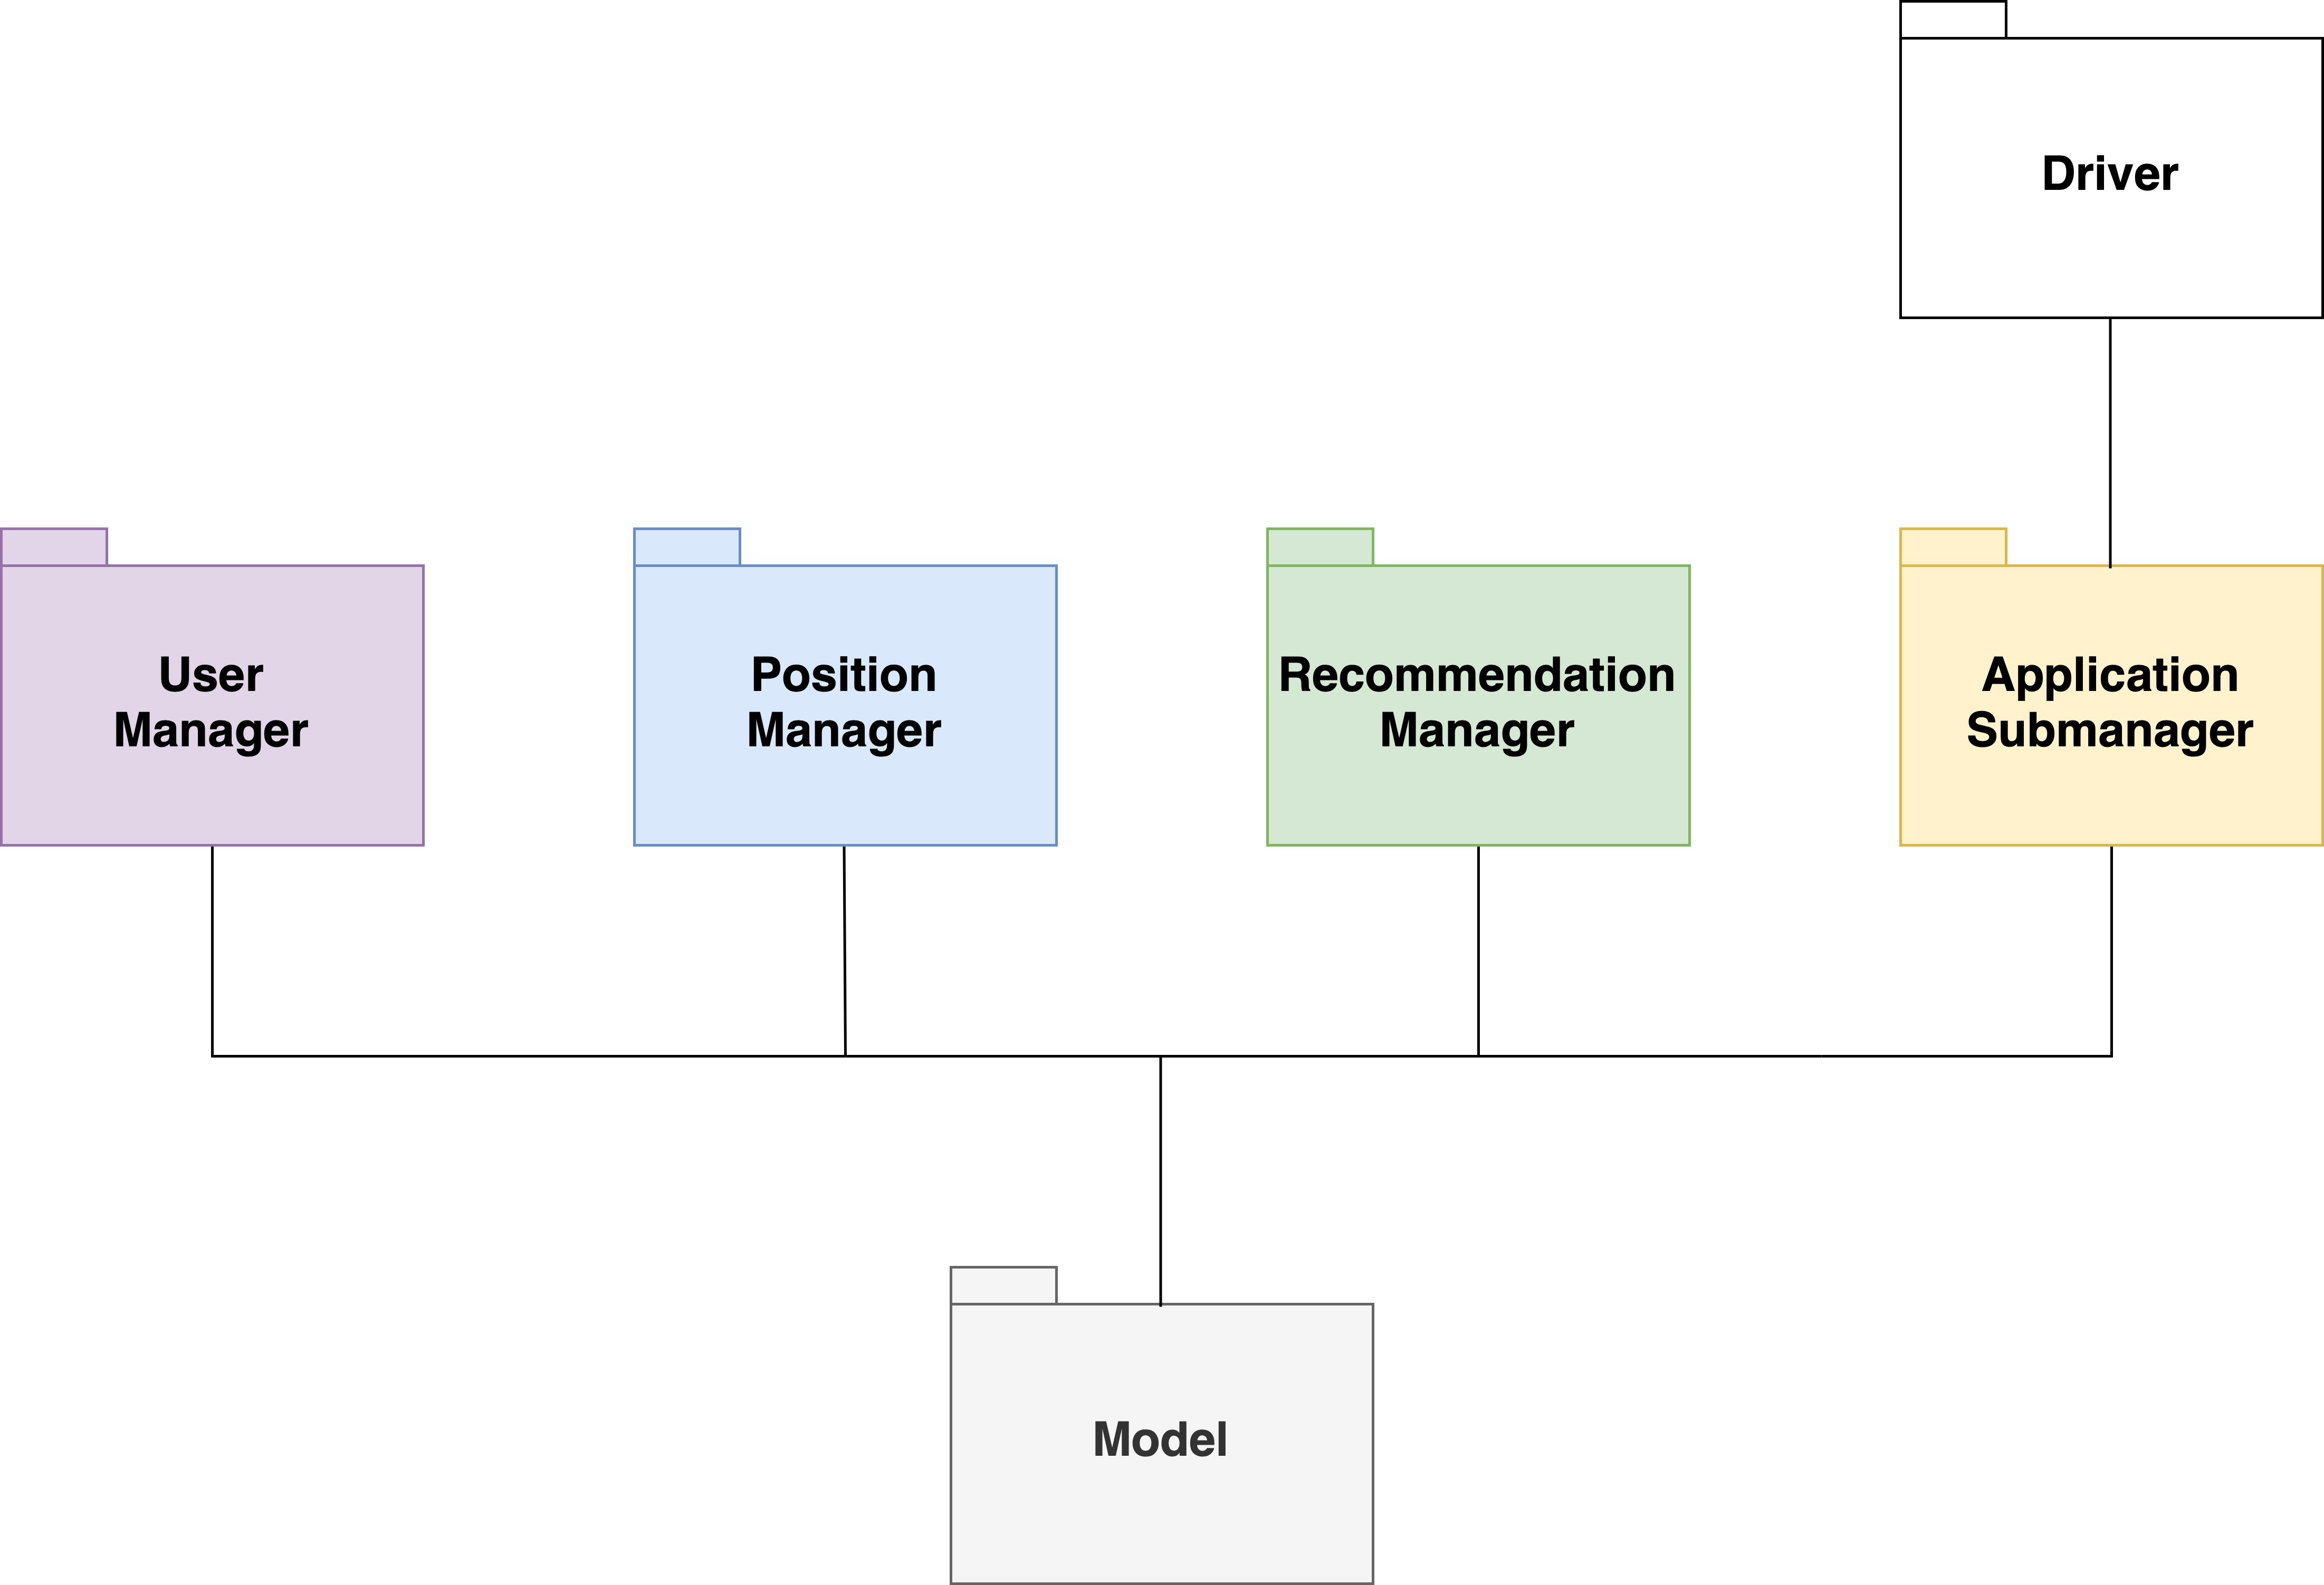
\includegraphics[width=13cm]{images/implementation-steps/7.png}
    \caption{Implementation step 7}
\end{figure}

\clearpage
The selection interview and questionnaire submanagers are integrated in the eighth step.

\begin{figure}[h]
    \centering
    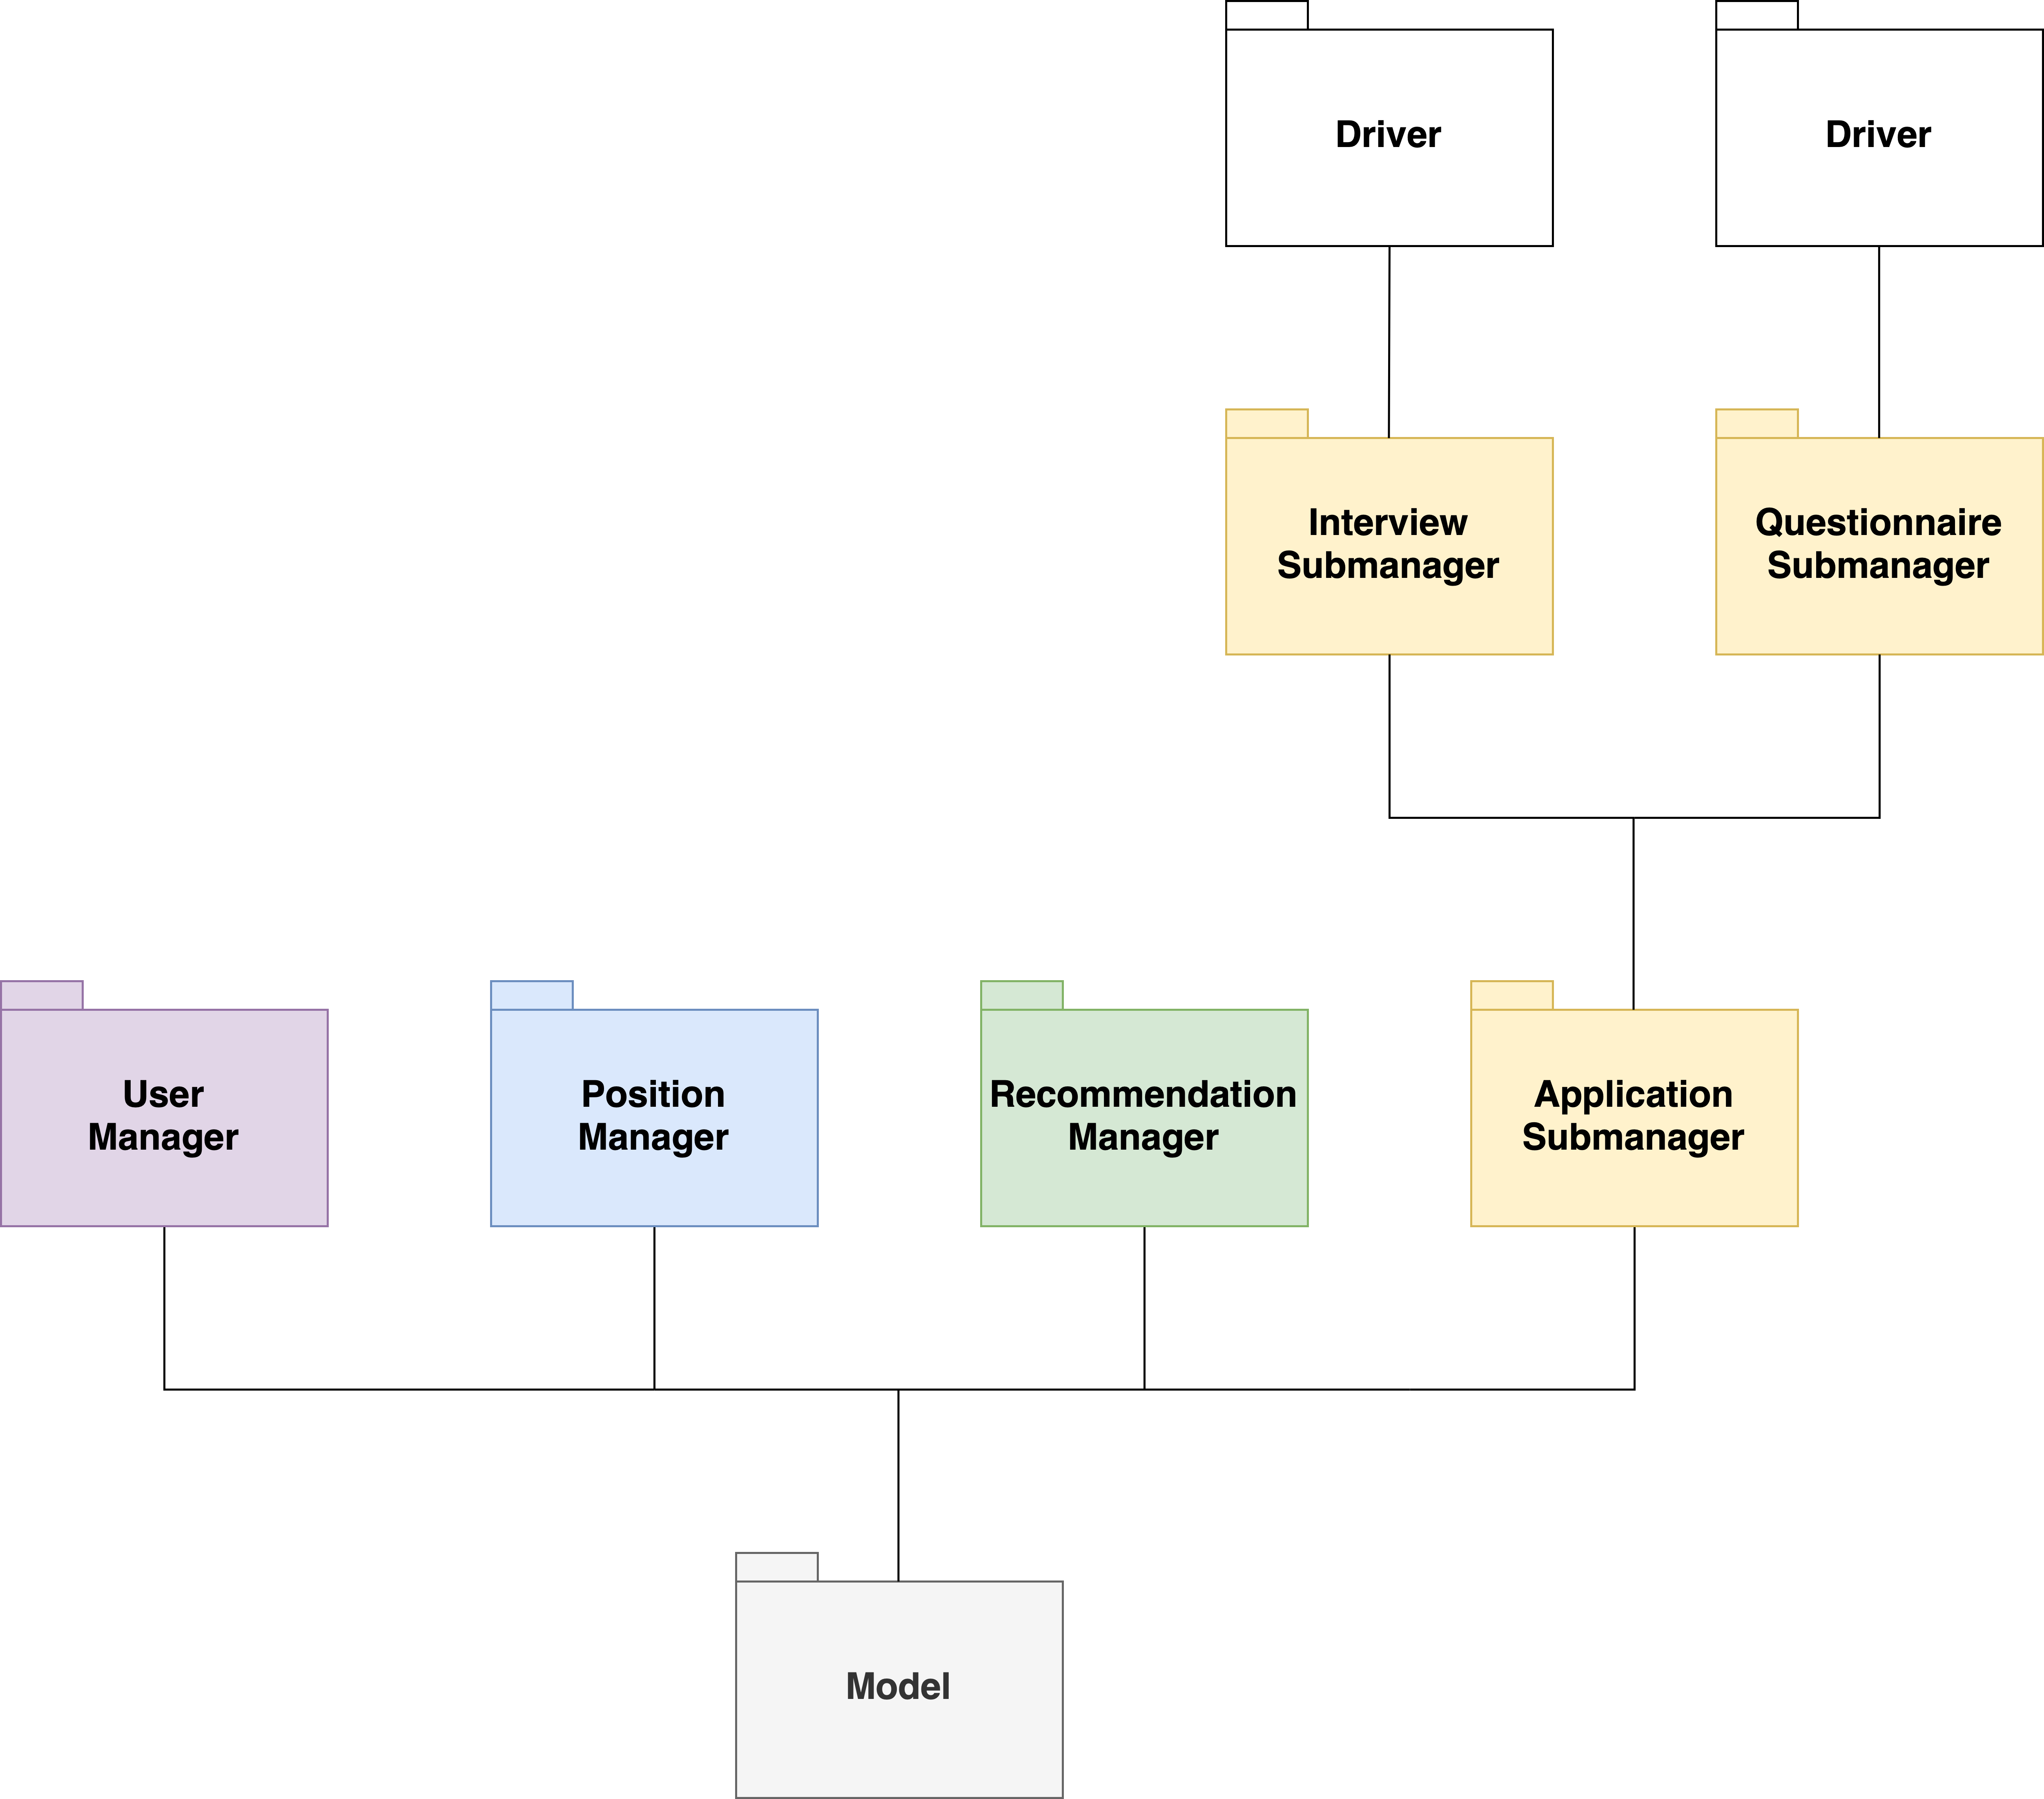
\includegraphics[width=14.5cm]{images/implementation-steps/8.png}
    \caption{Implementation step 8}
\end{figure}

\clearpage
The development proceeds to step nine with the application submanagers.

\begin{figure}[h]
    \centering
    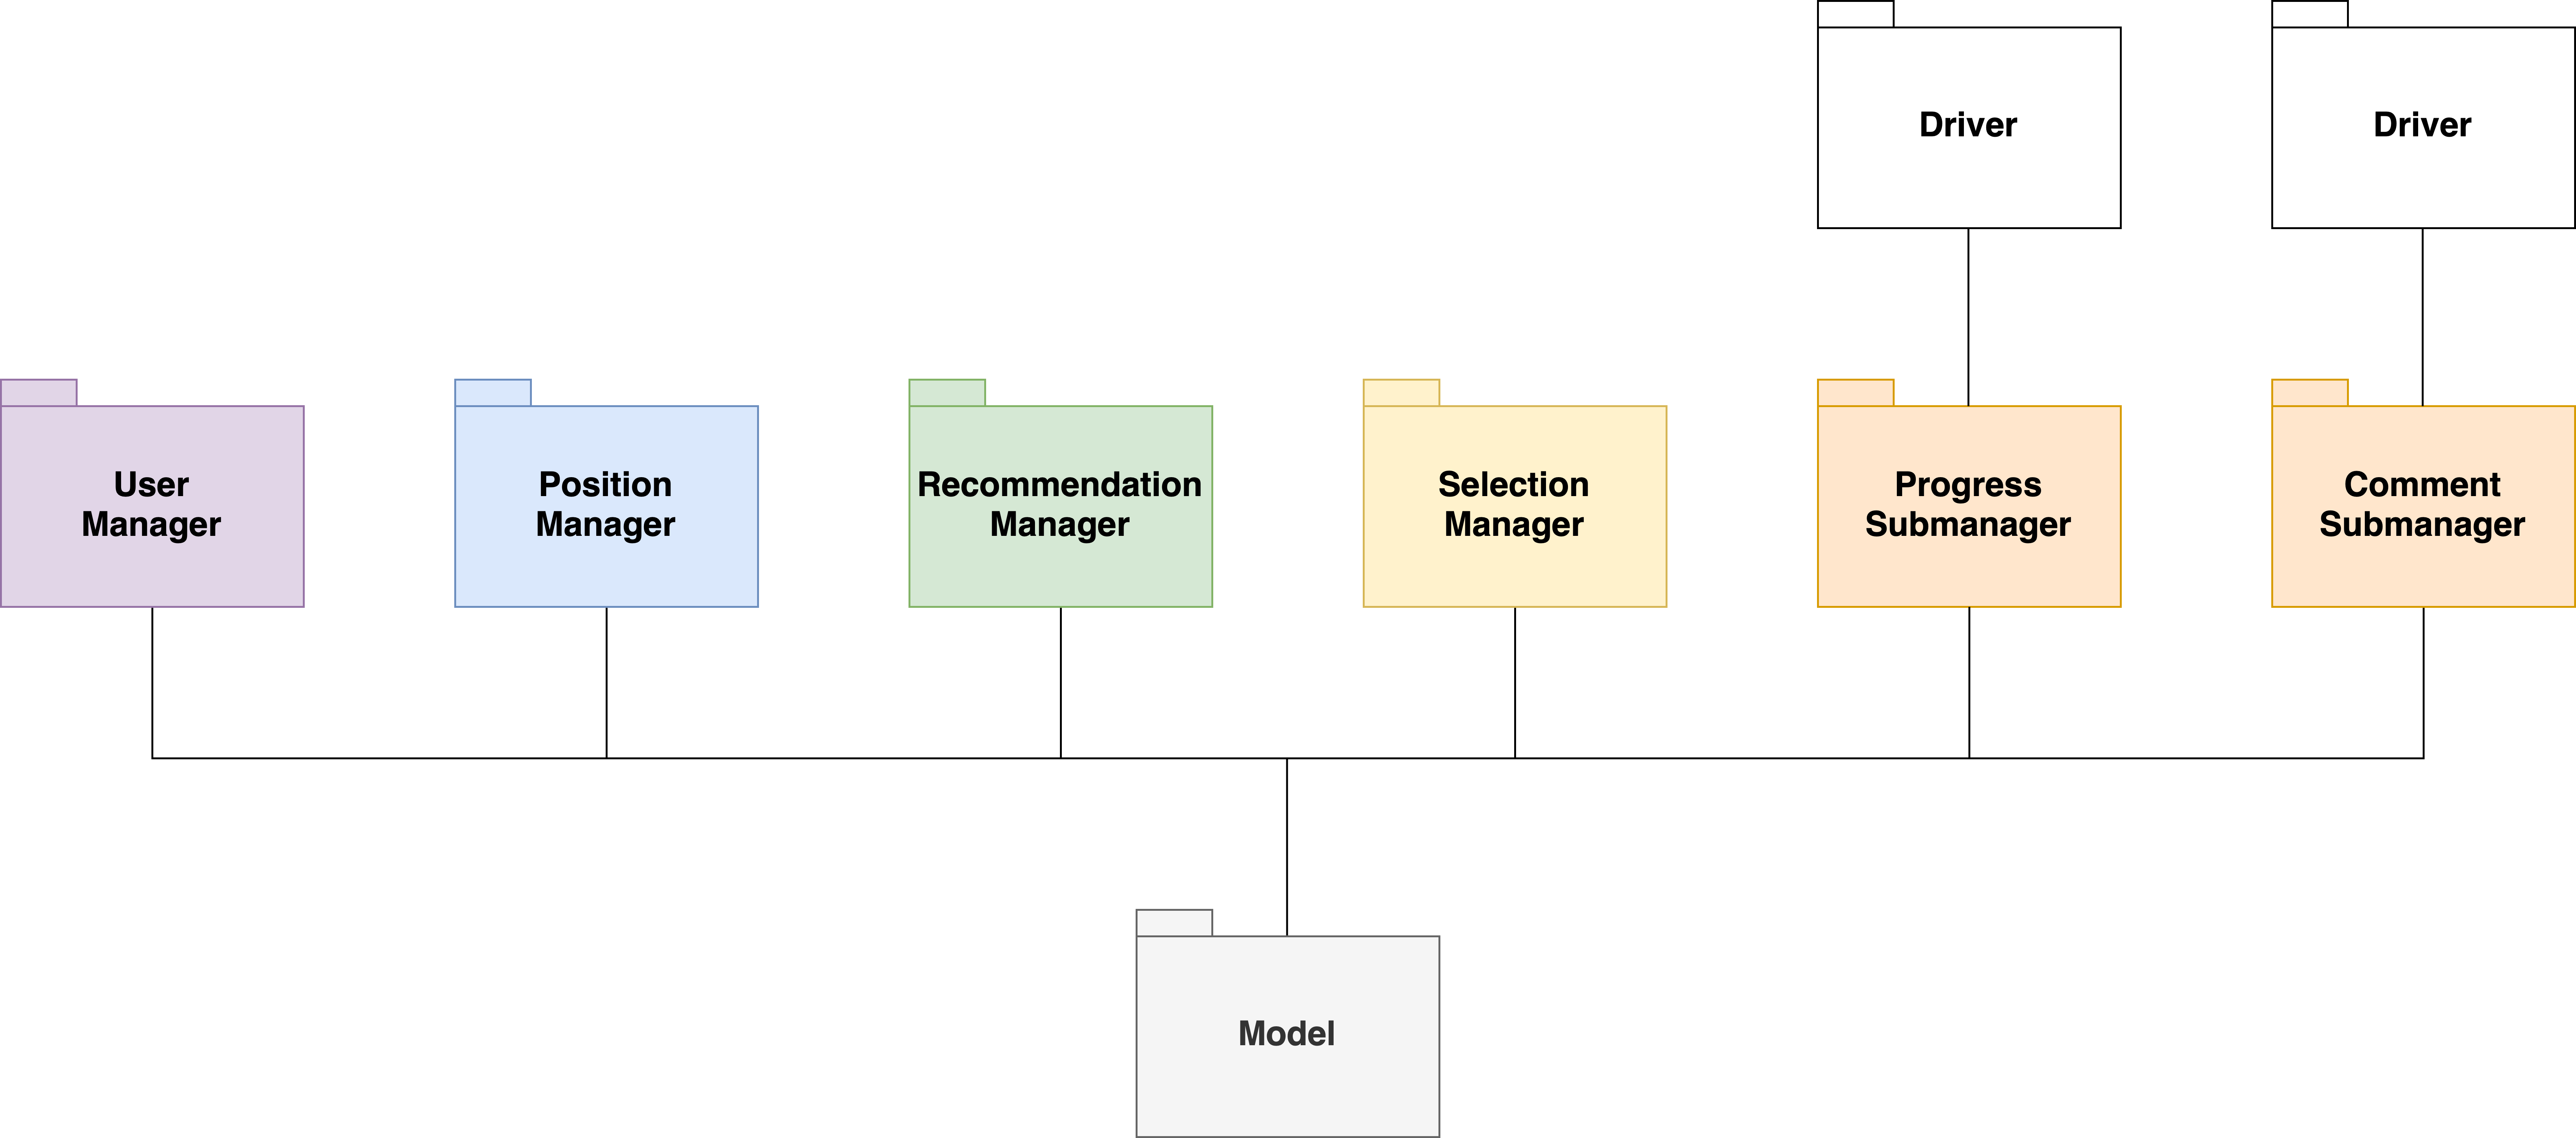
\includegraphics[width=16cm]{images/implementation-steps/9.png}
    \caption{Implementation step 9}
\end{figure}

Step ten applies the same pattern to the notification submanagers.

\begin{figure}[h]
    \centering
    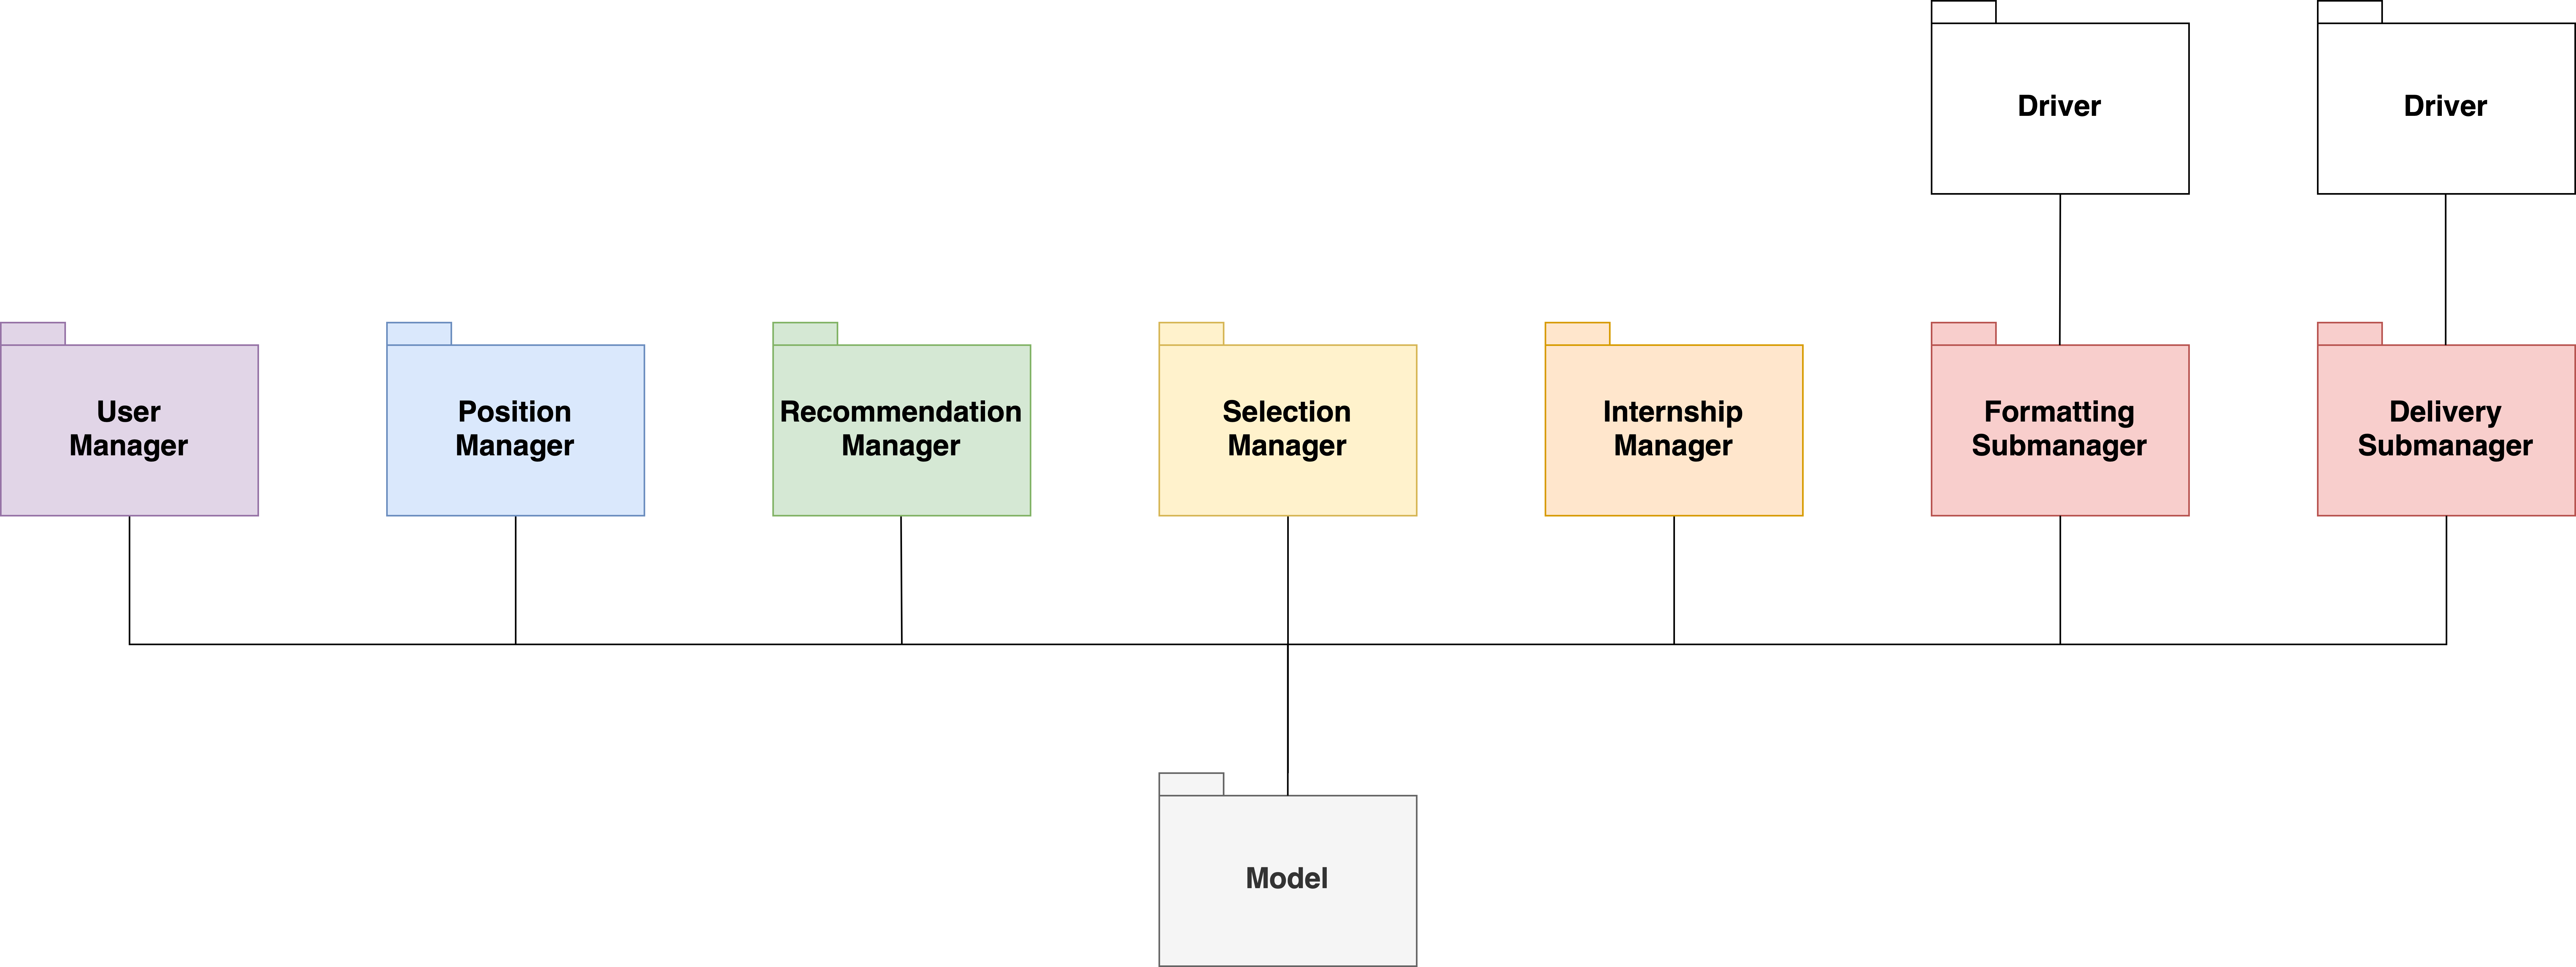
\includegraphics[width=16cm]{images/implementation-steps/10.png}
    \caption{Implementation step 10}
\end{figure}

\clearpage
Note that the notification manager supports all implemented managers.

\begin{figure}[h]
    \centering
    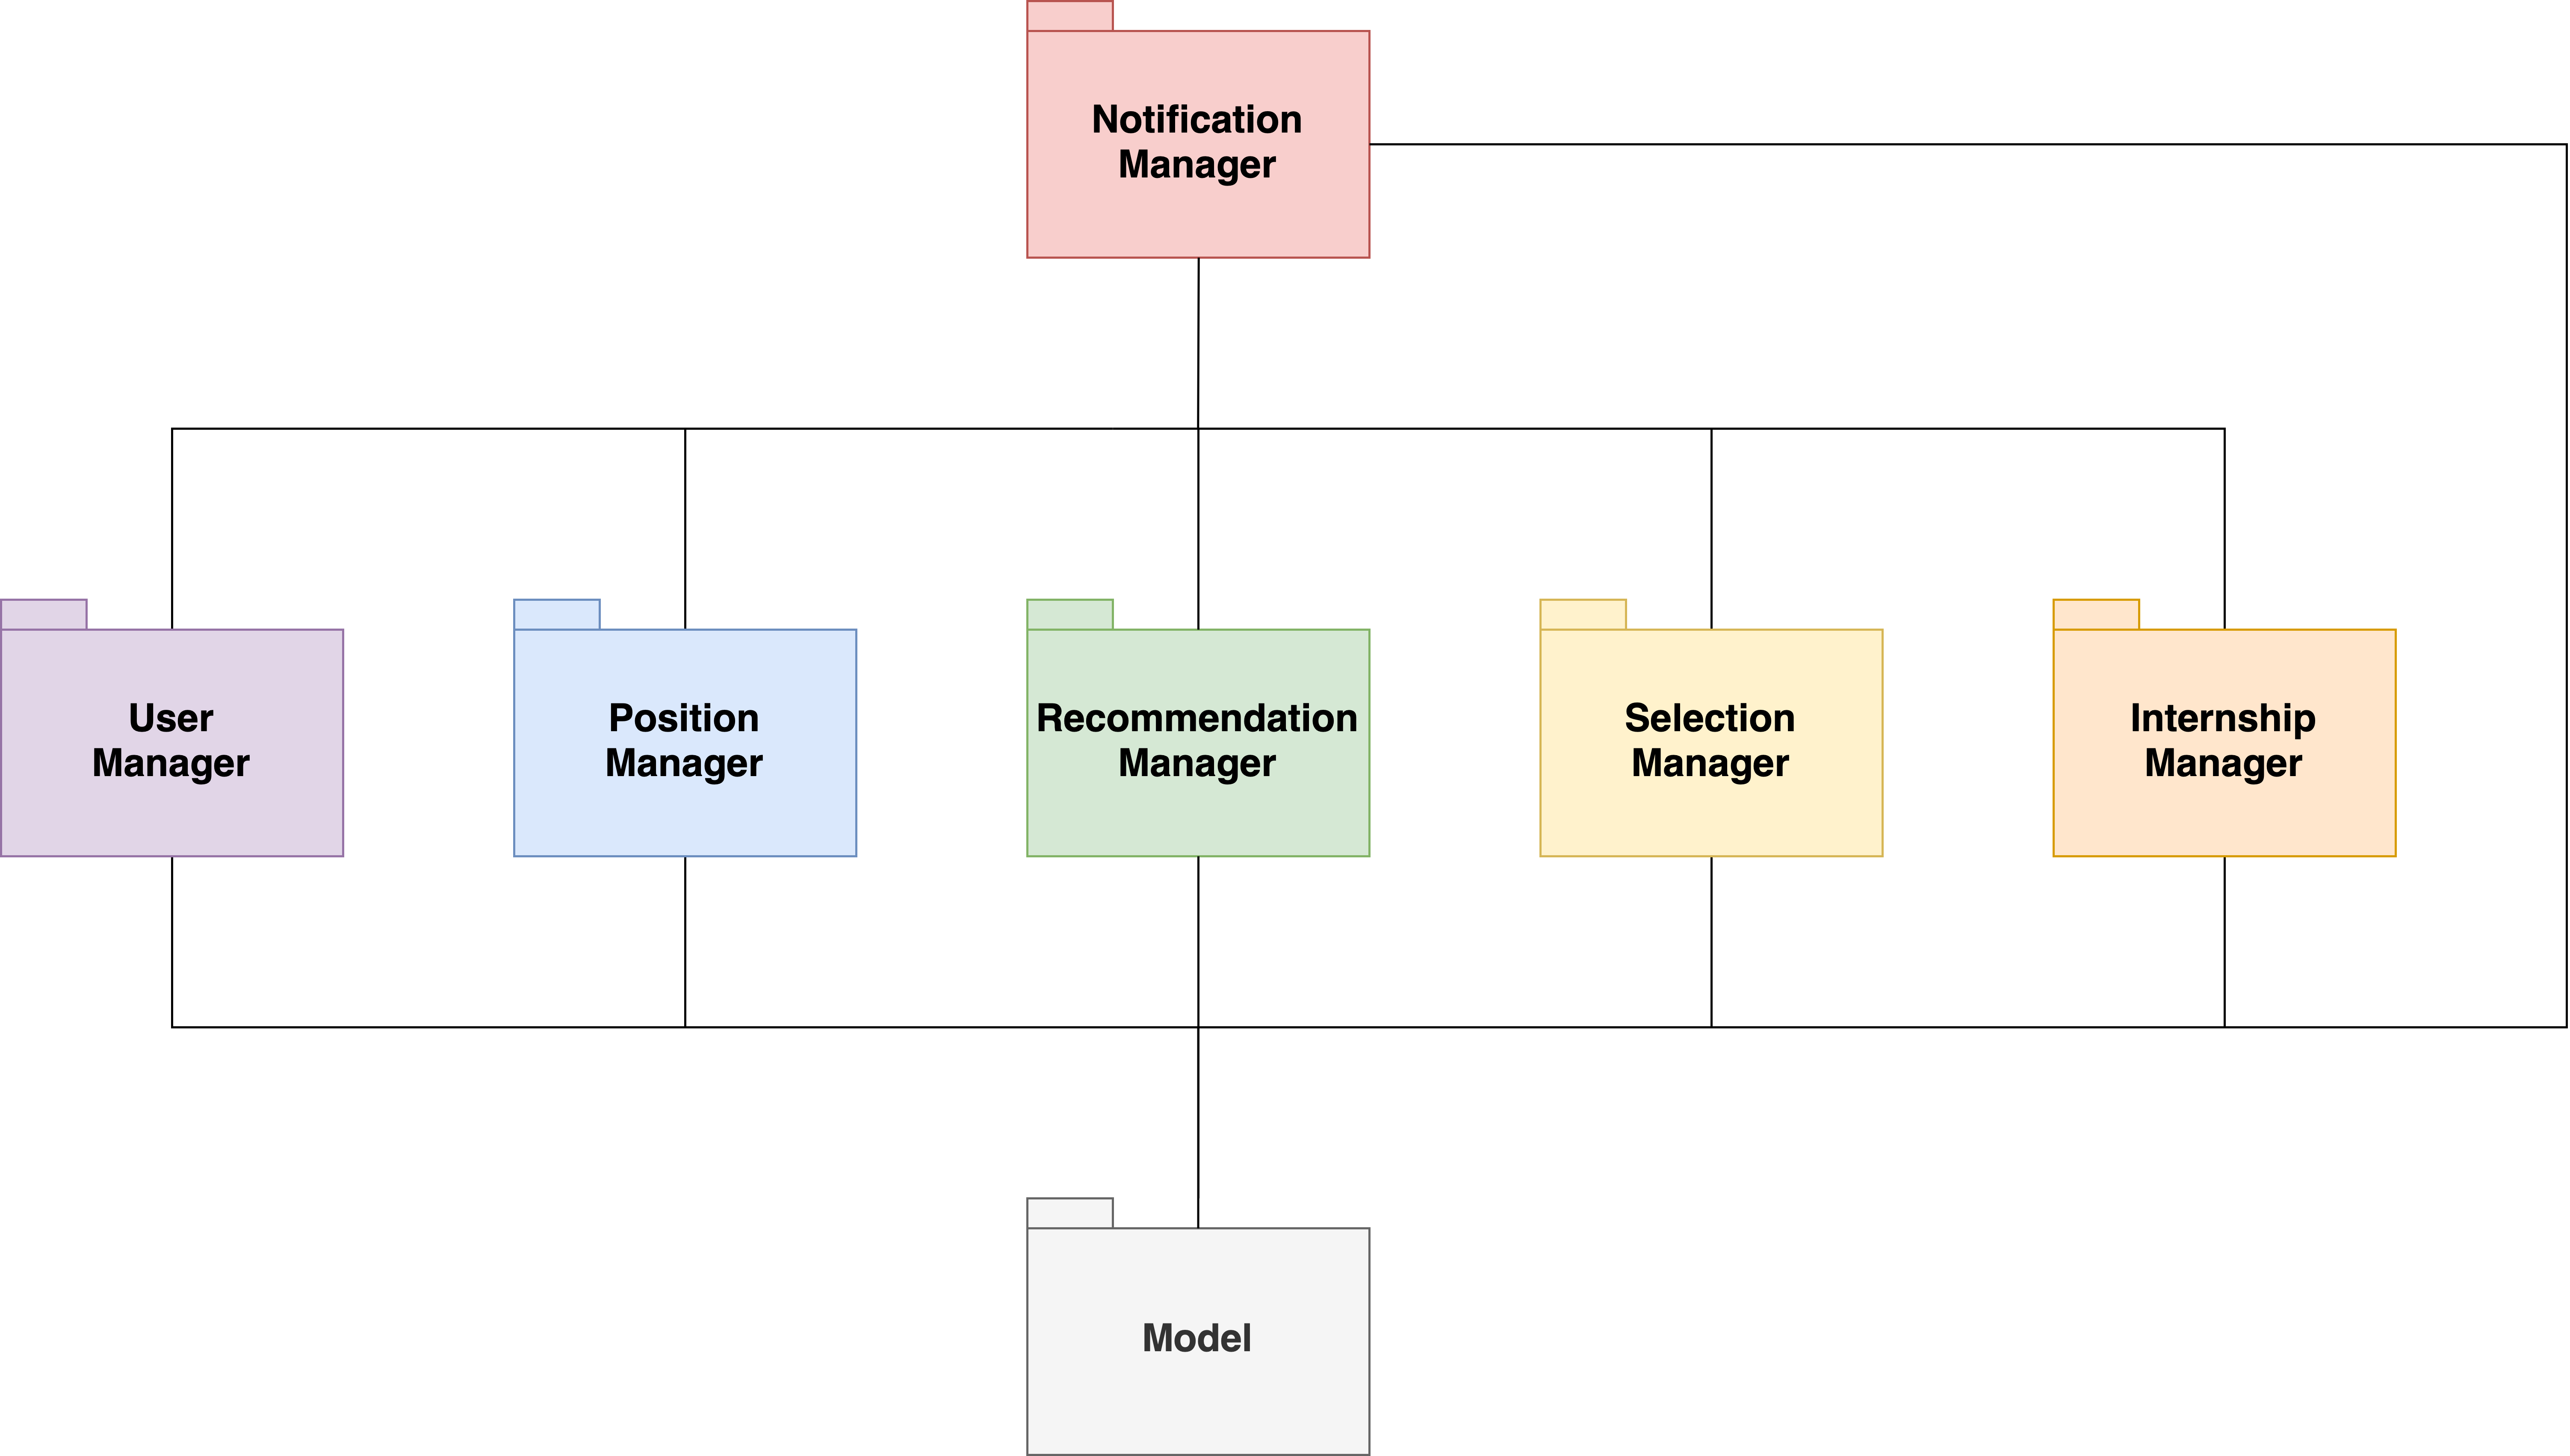
\includegraphics[width=16cm]{images/implementation-steps/11.png}
    \caption{Implementation step 11}
\end{figure}
